% Options for packages loaded elsewhere
\PassOptionsToPackage{unicode}{hyperref}
\PassOptionsToPackage{hyphens}{url}
\PassOptionsToPackage{dvipsnames,svgnames,x11names}{xcolor}
%
\documentclass[
  9pt,
  a4paper,
  DIV=11]{scrreprt}

\usepackage{amsmath,amssymb}
\usepackage{setspace}
\usepackage{iftex}
\ifPDFTeX
  \usepackage[T1]{fontenc}
  \usepackage[utf8]{inputenc}
  \usepackage{textcomp} % provide euro and other symbols
\else % if luatex or xetex
  \usepackage{unicode-math}
  \defaultfontfeatures{Scale=MatchLowercase}
  \defaultfontfeatures[\rmfamily]{Ligatures=TeX,Scale=1}
\fi
\usepackage{lmodern}
\ifPDFTeX\else  
    % xetex/luatex font selection
\fi
% Use upquote if available, for straight quotes in verbatim environments
\IfFileExists{upquote.sty}{\usepackage{upquote}}{}
\IfFileExists{microtype.sty}{% use microtype if available
  \usepackage[]{microtype}
  \UseMicrotypeSet[protrusion]{basicmath} % disable protrusion for tt fonts
}{}
\makeatletter
\@ifundefined{KOMAClassName}{% if non-KOMA class
  \IfFileExists{parskip.sty}{%
    \usepackage{parskip}
  }{% else
    \setlength{\parindent}{0pt}
    \setlength{\parskip}{6pt plus 2pt minus 1pt}}
}{% if KOMA class
  \KOMAoptions{parskip=half}}
\makeatother
\usepackage{xcolor}
\setlength{\emergencystretch}{3em} % prevent overfull lines
\setcounter{secnumdepth}{3}
% Make \paragraph and \subparagraph free-standing
\ifx\paragraph\undefined\else
  \let\oldparagraph\paragraph
  \renewcommand{\paragraph}[1]{\oldparagraph{#1}\mbox{}}
\fi
\ifx\subparagraph\undefined\else
  \let\oldsubparagraph\subparagraph
  \renewcommand{\subparagraph}[1]{\oldsubparagraph{#1}\mbox{}}
\fi


\providecommand{\tightlist}{%
  \setlength{\itemsep}{0pt}\setlength{\parskip}{0pt}}\usepackage{longtable,booktabs,array}
\usepackage{calc} % for calculating minipage widths
% Correct order of tables after \paragraph or \subparagraph
\usepackage{etoolbox}
\makeatletter
\patchcmd\longtable{\par}{\if@noskipsec\mbox{}\fi\par}{}{}
\makeatother
% Allow footnotes in longtable head/foot
\IfFileExists{footnotehyper.sty}{\usepackage{footnotehyper}}{\usepackage{footnote}}
\makesavenoteenv{longtable}
\usepackage{graphicx}
\makeatletter
\def\maxwidth{\ifdim\Gin@nat@width>\linewidth\linewidth\else\Gin@nat@width\fi}
\def\maxheight{\ifdim\Gin@nat@height>\textheight\textheight\else\Gin@nat@height\fi}
\makeatother
% Scale images if necessary, so that they will not overflow the page
% margins by default, and it is still possible to overwrite the defaults
% using explicit options in \includegraphics[width, height, ...]{}
\setkeys{Gin}{width=\maxwidth,height=\maxheight,keepaspectratio}
% Set default figure placement to htbp
\makeatletter
\def\fps@figure{htbp}
\makeatother
% definitions for citeproc citations
\NewDocumentCommand\citeproctext{}{}
\NewDocumentCommand\citeproc{mm}{%
  \begingroup\def\citeproctext{#2}\cite{#1}\endgroup}
\makeatletter
 % allow citations to break across lines
 \let\@cite@ofmt\@firstofone
 % avoid brackets around text for \cite:
 \def\@biblabel#1{}
 \def\@cite#1#2{{#1\if@tempswa , #2\fi}}
\makeatother
\newlength{\cslhangindent}
\setlength{\cslhangindent}{1.5em}
\newlength{\csllabelwidth}
\setlength{\csllabelwidth}{3em}
\newenvironment{CSLReferences}[2] % #1 hanging-indent, #2 entry-spacing
 {\begin{list}{}{%
  \setlength{\itemindent}{0pt}
  \setlength{\leftmargin}{0pt}
  \setlength{\parsep}{0pt}
  % turn on hanging indent if param 1 is 1
  \ifodd #1
   \setlength{\leftmargin}{\cslhangindent}
   \setlength{\itemindent}{-1\cslhangindent}
  \fi
  % set entry spacing
  \setlength{\itemsep}{#2\baselineskip}}}
 {\end{list}}
\usepackage{calc}
\newcommand{\CSLBlock}[1]{\hfill\break\parbox[t]{\linewidth}{\strut\ignorespaces#1\strut}}
\newcommand{\CSLLeftMargin}[1]{\parbox[t]{\csllabelwidth}{\strut#1\strut}}
\newcommand{\CSLRightInline}[1]{\parbox[t]{\linewidth - \csllabelwidth}{\strut#1\strut}}
\newcommand{\CSLIndent}[1]{\hspace{\cslhangindent}#1}

\usepackage{booktabs}
\usepackage{caption}
\usepackage{longtable}
\usepackage{colortbl}
\usepackage{array}
\makeatletter
\@ifpackageloaded{caption}{}{\usepackage{caption}}
\AtBeginDocument{%
\ifdefined\contentsname
  \renewcommand*\contentsname{Table des matières}
\else
  \newcommand\contentsname{Table des matières}
\fi
\ifdefined\listfigurename
  \renewcommand*\listfigurename{Graphiques}
\else
  \newcommand\listfigurename{Graphiques}
\fi
\ifdefined\listtablename
  \renewcommand*\listtablename{Tableaux}
\else
  \newcommand\listtablename{Tableaux}
\fi
\ifdefined\figurename
  \renewcommand*\figurename{\textbf{Graphique}}
\else
  \newcommand\figurename{\textbf{Graphique}}
\fi
\ifdefined\tablename
  \renewcommand*\tablename{\textbf{Tableau}}
\else
  \newcommand\tablename{\textbf{Tableau}}
\fi
}
\@ifpackageloaded{float}{}{\usepackage{float}}
\floatstyle{ruled}
\@ifundefined{c@chapter}{\newfloat{codelisting}{h}{lop}}{\newfloat{codelisting}{h}{lop}[chapter]}
\floatname{codelisting}{Listing}
\newcommand*\listoflistings{\listof{codelisting}{Liste des Listings}}
\captionsetup{labelsep=period}
\makeatother
\makeatletter
\makeatother
\makeatletter
\@ifpackageloaded{caption}{}{\usepackage{caption}}
\@ifpackageloaded{subcaption}{}{\usepackage{subcaption}}
\makeatother
\ifLuaTeX
\usepackage[bidi=basic]{babel}
\else
\usepackage[bidi=default]{babel}
\fi
\babelprovide[main,import]{french}
% get rid of language-specific shorthands (see #6817):
\let\LanguageShortHands\languageshorthands
\def\languageshorthands#1{}
\ifLuaTeX
  \usepackage{selnolig}  % disable illegal ligatures
\fi
\usepackage{bookmark}

\IfFileExists{xurl.sty}{\usepackage{xurl}}{} % add URL line breaks if available
\urlstyle{same} % disable monospaced font for URLs
\hypersetup{
  pdftitle={La Ville Compacte, une solution aux émissions de gaz à effet de serre},
  pdfauthor={Maxime Parodi; Xavier Timbeau},
  pdflang={fr},
  pdfkeywords={mobilité, choix modal, émissions de CO2, modèle à quatre
étapes, densité, forme urbaine},
  colorlinks=true,
  linkcolor={blue},
  filecolor={Maroon},
  citecolor={Blue},
  urlcolor={Blue},
  pdfcreator={LaTeX via pandoc}}

%%% title.tex we use to call other packages. Because this works
\usepackage{titlepic}
\usepackage{titling}
\usepackage{graphicx}
\usepackage{fontspec}
\usepackage{placeins}
\usepackage{graphbox}
\usepackage{tikz}
\usepackage{geometry}
\usepackage{xcolor}
\usepackage{amsmath}
\usepackage[some]{background}
\usepackage{lipsum}
\usepackage{caption}
\usepackage{datetime}
\usepackage{xstring}
\usepackage{blindtext}
\usepackage{scrlayer-scrpage}

\KOMAoptions{BCOR=5mm}
\setmainfont{OpenSans}[
  UprightFont = {*-Regular},
  BoldFont = {*-Bold},
  BoldItalicFont = {*-BoldItalic},
  ItalicFont = {*-Italic},
  Path = {_extensions/ofce/wp/OpenSans/},
  Extension = {.ttf}
]
\setsansfont{OpenSans}[
  UprightFont = {*-Regular},
  BoldFont = {*-Bold},
  BoldItalicFont = {*-BoldItalic},
  ItalicFont = {*-Italic},
  Path = {_extensions/ofce/wp/OpenSans/},
  Extension = {.ttf}
]

\def\getYear#1{\StrLeft{#1}{4}}
\def\getMonth#1{\StrMid{#1}{6}{7}}
\def\getDay#1{\StrRight{#1}{2}}

\def\jolimois#1{\monthname{\getMonth{#1}}}

\definecolor{quarto-callout-color}{HTML}{eeeeee}
\definecolor{quarto-callout-tip-color}{HTML}{dddddd}
\definecolor{quarto-callout-tip-color-frame}{HTML}{eeeeee}

\clearpairofpagestyles

\KOMAoptions{headsepline=true, twoside=true}

\pagestyle{scrheadings}
\setkomafont{pageheadfoot}{\small}

\rehead{Document de travail n°5-2024}
\lohead{\includegraphics[height=0.25cm]{www/ofce.png}}

\lofoot*{\thepage}
\refoot*{\thepage}
\begin{document}



\definecolor{ofcepbbleu}{RGB}{1, 97, 131}
\definecolor{ofcerouge}{RGB}{198, 45, 43}
\definecolor{scporouge}{RGB}{231, 0, 26}

\begin{titlepage}
  \backgroundsetup{
    scale=1,
    angle=0,
    opacity=1,
    contents={
  \begin{tikzpicture}[remember picture,overlay]
    \useasboundingbox (0,0) rectangle(\the\paperwidth,\the\paperheight);
      \node [anchor = center] at (-2.875-5.25,12.5) {\includegraphics[width=2.5cm]{www/ofce.png}};
      \node [anchor = center] at (-2.875-5.25,-12.75){\includegraphics[width=2.5cm]{\_extensions/ofce/wp/sciencespo.png}};
      \node [anchor = east] at (8.5,-11.5){\textcolor{black}{Date de première publication : 2024-01-30}};
      \node [anchor = east] at (8.5,-12){\textcolor{black}{Date de dernière modification : 2024-03-04}};
      \node [anchor = east] at (8.5,13-0.7){\textcolor{gray}{\Huge\textit{Working Paper}}};
      \draw [thick,black](-5.75,-13) -- (-5.75,13);
      \draw [color = white, fill=ofcepbbleu] (8.7,11.4) rectangle (10.45,13.15);
      \draw [color = white, fill=ofcepbbleu, very thick] (8.75-.5,11.25-.5) rectangle (8.75+.6,11.25+.6);
      \node [anchor = east] at (11-0.7,13-0.7){\textcolor{white}{\huge\textbf{5}}};
      \node [anchor = east] at (10-0.74,12-0.67){\textcolor{white}{\textbf{2024}}};
    \end{tikzpicture}
  }
}
\BgThispage

\hspace{4cm}
\begin{minipage}{12.5cm}
  \vspace{5cm}
  \begin{flushleft}
    \begin{spacing}{2.5}
      \textcolor{scporouge}{\Huge\textbf{\textsf{La Ville Compacte, une
solution aux émissions de gaz à effet de serre}}}
    \end{spacing}
    \vspace{20mm}
  \end{flushleft}
  
    
   \textbf{Maxime Parodi},           OFCE, Sciences Po Paris
   
   
   \textbf{Xavier Timbeau},           OFCE, Ecole Urbaine, Sciences Po
Paris
   
  % by-author
 \end{minipage}


%%
%% deuxieme page
\newpage
\pagestyle{empty}
\raisebox{-22cm}{
    \begin{minipage}[b]{40em}
      \textcolor{scporouge}{
        \textbf{CONTACT}}{

          \vspace{0.2cm}
          \vspace{0.2cm}
        
        \textbf{OFCE} 
  
        10 place de Catalogne 
        
        75014 Paris, FRANCE 
        
        Tel : +33 1 44 18 54 24
        
        \url{https://www.ofce.sciences-po.fr}
      }
    \end{minipage}
}
%%
%%
\newpage
%% troisieme page
\pagestyle{empty}
%%  \raisebox{3cm}{\begin{minipage}{\linewidth}
%%  \includegraphics[width=2cm]{www/ofce.png}
%%
%%  \includegraphics[width=2cm]{\_extensions/ofce/wp/sciencespo.png}
%%  \end{minipage}}
%%
 
\LARGE\textbf{La Ville Compacte, une solution aux émissions de gaz à
effet de serre}

\large\textbf{}

\vspace{1cm}


\par\rule{\textwidth}{0.5pt}

15005 mots.

\par\rule{\textwidth}{0.5pt}


\vspace{1cm}

\begin{flushright}
   \linespread{1}\small{\textbf{Maxime
Parodi}}, {\small{maxime.parodi@sciencespo.fr}}\par
   \linespread{1}\small{\textbf{Xavier
Timbeau}}, {\small{xavier.timbeau@sciencespo.fr}}\par
 % by-author
\end{flushright}
\end{titlepage}
\renewcommand*\contentsname{Table des matières}
{
\hypersetup{linkcolor=}
\setcounter{tocdepth}{0}
\tableofcontents
}
\setstretch{1.25}
\chapter{L'impératif d'un habitat
sobre}\label{limpuxe9ratif-dun-habitat-sobre}

Réduire les émissions de gaz à effet de serre est aujourd'hui un
objectif central des politiques publiques. Or, un tel objectif ne peut
être atteint sans agir à différents niveaux et dans de nombreux
domaines. Notamment, il ne va pas suffire de remplacer, au sein de notre
système de production d'énergie, les sources fossiles par des sources
renouvelables. Il faut aussi développer une stratégie de sobriété
énergétique, de manière à réduire le coût de la bascule vers des
énergies propres, à limiter l'empreinte environnementale liée à ces
investissements dans le système énergétique actuel et, également, à
éviter de produire de manière indirecte des émissions de gaz à effet de
serre.

L'un des principaux enjeux autour de la sobriété est lié à l'habitat et
à la mobilité des individus\,: quels modèles urbains promouvoir pour
éviter ou limiter les déplacements énergivores\,? Le \emph{Groupe
Intergouvernemental des Experts du Climat} (Lwasa, S. \emph{et al.},
2022~; Seto \emph{et al.}, 2014) a ainsi réaffirmé que la ville compacte
est un des grands leviers de la transition vers des sociétés neutres en
carbone. Cette position s'inscrit dans un long débat aussi bien aux
Etats-Unis, où les défenseurs de la ville compacte s'opposent à
l'étalement urbain (Ewing (1997) vs Gordon et Richardson (1997); Newman
et Kenworthy (1989a)), qu'en Europe (Jenks, Williams et Burton, 1996) ou
en Chine (Pan, Shen et Zhang, 2009) pour ne citer que quelques exemples
emblématiques.

L'endroit où vivent les individus conditionne leurs émissions de gaz à
effet de serre par deux canaux principaux\,: d'une part, les émissions
liées au logement, au moment de sa construction puis celles induites par
ses dépenses énergétiques, principalement le chauffage. D'autre part, la
mobilité quotidienne pour accéder à l'emploi, à l'éducation et à toutes
les aménités dont les ménages ont l'usage. On pourrait ajouter des liens
plus difficiles à mettre en évidence entre le lieu de résidence et les
comportements de consommation. Ainsi, l'effet «\,barbecue\,» ou
«\,hypothèse de compensation\,» (Holden et Norland, 2005~; Massot et
Orfeuil, 2007~; Muñiz, Calatayud et Dobaño, 2013~; Orfeuil et Soleyret,
2002) voudrait que les ménages urbains se déplacent moins la semaine
mais ont un besoin de nature ou un besoin de fuir la ville qui les
conduit à faire plus de déplacements de loisirs les week-ends ou pendant
les vacances. Une fois contrôlé des plus importantes variables
socio-économiques, un ménage urbain prend effectivement plus souvent
l'avion pour les vacances et, plus marginalement, effectue des
déplacements plus longs le week-end qu'un ménage vivant à la campagne.
Toutefois, les citadins n'effectuent pas ces déplacements pour
satisfaire un besoin de nature ou pour fuir la ville, puisque les
destinations sont souvent d'autres villes (Munafò, 2017). La mobilité
occasionnelle des citadins doit plus s'interpréter comme la traduction
de leurs goûts pour les expériences diverses, contrastées et
cosmopolitiques, qui expliquent leur désir de vivre dans des centres
urbains. Il reste que la hausse des kilomètres attribuables à cet effet
«\,barbecue\,» est marginal (un facteur 10) en regard de la différence
de kilomètres parcourus entre un ménage urbain et un ménage rural. Il
faudrait également tenir compte du cas d'un ménage s'éloignant de
l'emploi mais qui compense en télétravaillant. Pour l'heure, il est
encore difficile de dresser un réel bilan kilométrique de ces cas
(Cervero, 1989~; Orfeuil et Soleyret, 2002).

Les postes «\,mobilité\,» et «\,logement\,» couvrent plus de 50\% de
l'empreinte carbone des ménages. Selon le SDES (Baude, 2022), la
mobilité représentait 30\% de l'empreinte carbone d'un français en 2017.
L'empreinte carbone inclue les émissions directes et indirectes et
s'élevait en 2017 à 9,5~tCO\textsubscript{2}eq/an par habitant en
France. Les émissions liées au logement représentent 23\% de l'empreinte
totale. L'empreinte carbone de la mobilité se décompose en 60\% (18\% de
l'empreinte totale) d'émissions directes par la combustion de fossiles,
19\% (5,7\% de l'empreinte) pour la construction et l'entretien des
véhicules. Le transport aérien compte pour 10\% (6\% de l'empreinte). La
part restante (11\% et 6,6\% de l'empreinte) est liée aux services de
transport directs ou indirects que les ménages consomment (Baude, 2022,
p.~16).

L'enjeu est donc clair et les leviers sont nombreux (Hsu \emph{et al.},
2023). Pour les consommations résidentielles\,: une plus grande
efficacité thermique des bâtiments, des températures cibles plus basses
l'hiver, un moindre recours à la climatisation l'été et une moindre
utilisation de l'eau chaude. Pour la construction des bâtiments\,: la
décarbonation de la construction, des normes d'efficacité énergétique
pour les nouveaux bâtiments, une limitation des constructions nouvelles,
l'utilisation du bâti existant ou le partage du bâti existant en
réduisant l'espace alloué par personne ou en multipliant les usages d'un
local au cours d'un cycle. Pour les mobilités\,: l'électrification des
véhicules, la hausse de l'occupation moyenne des véhicules (covoiturage,
transport en commun), le passage à des mobilités douces (vélo ou marche)
et, enfin, la réduction des distances parcourues, soit par la baisse de
la fréquence des trajets, soit par le raccourcissement des trajets en
habitant plus près des emplois et services.

Le modèle de la ville compacte (Jenks, Williams et Burton, 2003) paraît
répondre à chacun de ces enjeux en combinant l'utilisation de nombreux
leviers. En regroupant activités et résidents, la forme urbaine réduit
\emph{a priori} les distances, fournit les services et les activités
dans un voisinage accessible sans voiture, permet des transports en
commun rentables et denses et réduit de nombreux coûts (entretien des
routes et des réseaux en tout genre, services de livraison, gestion des
déchets, etc.). Toutefois, ce modèle urbain a ses adversaires, qui
interprètent celle-ci sous des formes repoussantes (tours gigantesques,
espace privé minuscule, etc.) comme si la compacité ne pouvait se
matérialiser que d'une unique façon. Depuis l'invention du terme
(attribué à Dantzig, Dantzig et Saaty, 1973), la controverse entre un
modèle de ville fondé sur l'usage de la voiture, dans lequel les gains
de vitesse apporté par la technologie invitent à l'étalement, et un
modèle organisé pour exclure la voiture des mobilités quotidiennes est
vive.

Cette controverse a, au cours des 50 dernières années, pris plusieurs
formes. La notion de ville fonctionnelle (dans la lignée de Janes Jacob
(Jacobs, 1961) et contre Le Corbusier) a trouvé dans le \emph{New
Urbanism} un argument fondé sur les préférences des individus et le
développement organique des villes, poussé par les besoins des
habitants. L'étalement urbain serait alors une manifestation d'un désir
d'être entre-soi de certains groupes sociaux\,: ainsi des riches évitant
les pauvres et des blancs fuyant les noirs (Levine, 2010). La question
climatique, par l'injonction à la sobriété, est un autre terrain
d'affrontement entre ces deux visions radicales de la ville. Cet
affrontement prend une nouvelle dimension en opposant non plus seulement
étalement urbain et ville compacte, mais aussi ville compacte et mode de
vie sobre avec une faible division du travail et une grande
autonomie\,-- parfois appelé décroissance ou post-croissance urbaine
(Savini, Ferreira et von Schönfeld, 2022).

Outre la question climatique, l'usage la voiture, notamment thermique,
au sein des villes apporte son lot de problèmes\,: pollution de l'air,
congestion, accidents de la route, qui tous impactent négativement la
santé humaine. Dans un contexte de hausse des coûts relatifs de
l'énergie à court et à long terme, les mobilité quotidiennes et la
consommation d'énergie résidentielle exercent une contrainte de plus en
plus importantes sur les budgets des ménages. La répartition spatiale
étant conditionnée notamment par les prix de l'immobilier, les choix de
localisation peuvent être fait sans pouvoir anticiper correctement les
évolutions des coûts futurs et induire un enfermement de certaines
populations, souvent modestes, dans des zones excentrées qui finiront
par entraîner des coûts de transport difficilement soutenables. La
facilité d'accès à l'emploi et à d'autres aménités en fonction de son
lieu de résidence\,--- que l'on peut mesurer par l'accessibilité\,---
détermine les pratiques de mobilités des résidents\,: les modes de
transport possibles, les coûts de chaque trajets, l'activité physique
induite, ou encore la possibilité pour des individus ne pouvant pas
conduire (comme les plus jeunes) d'accéder aux aménités de manière
autonome.

L'argument environnemental pour les villes compactes repose sur une
empreinte carbone plus faible pour des déplacements plus courts et plus
doux que dans le cas de l'étalement urbain ou dans le cas d'une
mégalopole où les distances s'allongent malgré une densité importante.
Dans ce débat, une littérature assez récente (depuis les années 2000) a
versé un grand nombre d'arguments empiriques en utilisant les données de
grandes enquêtes auprès des ménages sur les mobilités. Il en ressort un
diagnostic mitigé\,: une plus grande densité est bien associée à de
moindres déplacements, mais cette conclusion est fragile en raisons de
nombreuses difficultés méthodologiques (liées à l'endogénéité des
variables et à des biais de sélection). Plus encore, l'effet identifié
semble faible\,-- une élasticité de -0,1 entre densité et nombre de
kilomètres parcourus\,-- au point qu'il est illusoire de compter sur la
hausse de la densité pour réduire les émissions Duranton et Turner
(2018).

Nous présentons dans la section suivante cette littérature, les
principaux résultats ainsi qu'une analyse critique des méthodes qui
conduisent au résultat principal. Nous présenterons ensuite une approche
alternative, s'attachant à mieux définir la notion de densité et surtout
à préciser ce qu'augmenter la densité veut dire, pour montrer qu'il
s'agit bien d'une levier efficace pour réduire les émissions liées à la
mobilité, conformément à l'intuition initiale de Newman et Kenworthy.

\chapter{Une densité plus élevée fait-elle baisser les
émissions\,?}\label{sec-densemis}

Le lien entre la géographie, la forme urbaine et les mobilités
résidentielles a donné lieu à un débat nourri, vieux de quelques
décennies et persistant. Tout le monde a en tête les travaux et le
graphique de Newman et Kenworthy (graphique~\ref{fig-newmankenworthy})
(Newman et Kenworthy, 1989a, 1989b, 1999) représentant une corrélation
négative entre consommation d'énergie annuelle de carburant et densité,
qui a confortée l'intuition que les villes compactes sont plus
soutenables que les villes «\,étalées\,». Le graphique de (Newman et
Kenworthy, 1999) a été largement critiqué et la corrélation affichée sur
le graphique a été jugée en partie fallacieuse du fait de nombreux
facteurs, dont le niveau de développement de chacune des villes
considérées, le prix local du carburant ou d'autres facteurs explicatifs
communs (Ewing \emph{et al.}, 2017). En 2015, Ewing et Hamidi (2015)
recensaient plus de 200 études empiriques et 12 revues de littérature
sur ce sujet. Plusieurs éléments à la fois théoriques, méthodologiques
et empiriques ont été raffinés et conduisent à un résultat pour le moins
mitigé selon lequel l'influence de la densité ou d'autres dimensions de
la forme urbaine sur les consommations de carburant seraient trop petits
pour jouer un rôle prépondérant dans la réduction des émissions de gaz à
effet de serre.

\begin{figure}

\caption{\label{fig-newmankenworthy}Lien entre densité moyenne et
consommation de carburant par villes (Newman\&Kenworthy 1989)}

\centering{

\includegraphics[width=3.3125in,height=\textheight]{images/newmankenworthy.png}

}

\end{figure}%

Ainsi, l'affirmation initiale s'est trouvé «\,anesthésiée\,» et il
faudrait croire que le lien entre densité et empreinte carbone est trop
faible pour justifier une politique urbaine. Une telle anesthésie a été
possible parce que la densité est plutôt un mauvais indicateur de la
forme urbaine\,; c'est un indicateur équivoque. Les critiques
méthodologiques de l'article de Newman et Kentworthy sont certes
justifiées, mais leur intuition exige un examen qui ne se limite pas à
redéfinir la mesure de la densité urbaine. Par exemple, des
quantification centrées sur l'accessibilité à l'emploi ont un meilleur
pouvoir explicatif. Mais, plus encore, il faudrait surtout démêler deux
questions\,: celle de savoir si toute densification, en général,
entraîne nécessairement une réduction des émissions\,-- la question qui
a monopolisé l'attention\,-- et celle de savoir quels scénarios de
densification apportent un niveau de réduction suffisant pour justifier
une politique publique.

\section{Quantifier la forme urbaine}\label{quantifier-la-forme-urbaine}

La densité de population, l'indicateur retenu par Newman et Kenworthy
(1989a), ne suffit pas à décrire la forme et la structure des villes. La
même distribution spatiale de la densité peut cacher des formes urbaines
très diverses. Depuis Cervero et Kockelman (1997), les indicateurs
complémentaires à la densité ont été catalogué et sont généralement
appelés les D. Aux 3 D initialement proposés par Cervero et Kockelman,
pour \textbf{D}ensité, \textbf{D}iversité et \textbf{D}esign, ont été
ajouté d'autres D comme la distance au centre des emplois
(\textbf{C}entral \textbf{B}usiness \textbf{D}istrict) ou la distance
aux transports en commun (le plus proche, un indicateur de connectivité,
etc\ldots). Une plus grande densité devrait induire moins de kilomètres
parcourus par résident, du moins si l'on mesure la densité à la bonne
échelle, de manière à rendre compte de la proximité des centres
d'intérêt des résidents.

Le terme «\,densité\,» recouvre ainsi différentes notions\,: la densité
peut être celle des habitants, des logements, des bâtiments ou de la
surface habitable. Elle peut être calculée à différentes échelles et
éventuellement lissée, conduisant à des résultats sensiblement
différents puisque les tissus urbain sont toujours très hétérogènes sur
un territoire donné. La façon la plus immédiate de calculer la densité
est de prendre le ratio entre le nombre d'habitants et la surface bâtie,
pour une zone donnée, mais il est également possible de calculer la
densité moyenne en pondérant la densité sur une maille (régulière ou
non) par le nombre d'habitants résidents dans cette maille. Cette
densité pondérée par la population (PWD), parfois appelée «\,densité
articulée\,», rend mieux compte de la densité moyenne ressentie par les
résidents. Par exemple, la densité moyenne simple de New York dans son
ensemble est plus faible que celle de Los Angeles alors que la densité
pondérée par la population met New York au dessus de Los Angeles en
termes de densité, puisque les résidents de Manhattan sont nombreux a
percevoir que la densité de Manhattan est forte.

Le deuxième D\,--- la diversité\,--- cherche à tenir compte de la
spécialisation de l'environnement urbain. Dans beaucoup de villes
américaines, du fait d'une politique persistante de zonage peu pratiquée
en Europe (Hirt, 2012), les espaces sont spécialisés, en particulier
entre zones de résidences et de commerce ou d'activité économique. La
diversité, mesurée par exemple par (l'opposé d') un indice de
Herfindahl, permet de rendre compte de l'imbrication des services ou des
opportunités d'emplois avec les lieux de résidence. Là encore, l'échelle
de prise en compte de la diversité est un point important et, à nouveau,
l'imbrication peut être pondérée pour mieux rendre compte des
perceptions. Tout comme pour la densité, on s'attendrait à ce qu'une
plus grande diversité soit associée à moins de kilomètres parcourus.

Le troisième D\,--- le design\,--- fait référence à la configuration des
rues, des routes ou du réseau de transport. Une configuration de routes
peu denses, composé d'axes traversant continus et à fort débit est peu
propice à la marche. Un réseau de ruelles entourant des blocs de
bâtiments plus petits permet au contraire une circulation capillaire. La
mesure du design passe par des indicateurs variés comme le nombre
d'intersection, la taille des blocs. Alternativement, (Blaudin de Thé,
Carantino et Lafourcade, 2021) utilisent la dimension fractale des
bâtiments\footnote{La dimension fractale est définie comme la pente du
  ratio entre le nombre de bâtiments et le nombre de pavés lorsque la
  taille du pavage varie et tend vers 0 (éventuellement en \(log\)).}.

La distance au centre des emplois (CBD) est une mesure assez simple dès
lors qu'on peut identifier facilement le centre de l'emploi.
Malheureusement, le modèle monocentrique qui justifierait cette mesure
décrit très mal la plupart des villes et elle est très insatisfaisante
dans le cas général. Malgré cela, le nombre de kilomètres voyageurs
(VKT) est corrélé fortement à ce type de mesure (voir plus bas).

La distance aux transports en commun est également simple
conceptuellement. On retient généralement la distance au plus proche
arrêt de transport en commun ou le nombre d'arrêt dans un périmètre
donné (par exemple 10 minutes de marche). C'est toutefois un indicateur
assez frustre puisqu'il ne suffit pas de résider près d'une station de
métro ou d'un arrêt de bus, il faut encore que le transport desserve les
bonnes destinations aux bons moments. Ceci dit, cette mesure est
renseignée dans les enquêtes de mobilité (comme l'\textbf{E}nquête
\textbf{M}obilité \textbf{C}ertifiée \textbf{C}EREMA, EMC2) et elle peut
être intéressante une fois associée aux données sur les réseaux de
transports (de type GTFS).

En décrivant la forme urbaine par ces grandeurs, on dispose
d'indicateurs qui sont principalement locaux et associés à l'endroit de
résidence. Ils peuvent être calculés à différentes échelles, comme dans
l'analyse multiniveaux de Lee et Lee (2020), mais aucun de ces
indicateurs n'éclaire réellement la capacité systémique des
infrastructures d'une ville à relier les résidents à leurs lieux
d'intérêt, emplois ou aménités.

\section{Endogénéité et autosélection des
résidents}\label{endoguxe9nuxe9ituxe9-et-autosuxe9lection-des-ruxe9sidents}

Bien qu'il soit délicat de tirer une conclusion simple et univoque du
large panel d'analyses sur le lien entre densité et émissions, des
mesures de la forme urbaine comme la densité d'habitants ou d'emploi,
parfois des mesures plus complexes comme la dimension fractale du bâti
(Blaudin de Thé, Carantino et Lafourcade, 2021), la diversité locale de
l'emploi, des indicateurs de centralité, de connectivité ou de
continuité (Ewing et Hamidi, 2015) sont corrélées négativement avec le
nombre de kilomètres-voyageurs (abrégé en VKT pour
\emph{\textbf{V}ehicule \textbf{K}ilometers \textbf{T}raveled} ou
\emph{\textbf{V}ehicule \textbf{M}iles \textbf{T}raveled} dans la
littérature en langue anglaise).

L'évaluation du lien causal demeure délicate en raison de possibles
biais de sélection des résidents\,: dans quelle mesure les ménages qui
de moindres revenus et se trouvent contraints à des déplacements plus
courts et non motorisés habitent-ils des zones plus denses et des
logements plus petits et plus proches du centre-ville\,? Ou encore, les
individus effectuent-ils de longs trajets en voiture parce qu'ils
habitent loin ou, à l'inverse, est-ce qu'ils résident loin parce qu'ils
aiment faire de la voiture\,? Autant de questions qui fragilisent
l'établissement d'un lien causal entre densité et VKT. En général, dans
ces études, la corrélation est considérée en partie comme causale mais
faible. (Duranton et Turner, 2018) concluent ainsi pour les Etats-Unis à
une élasticité de l'ordre de -0.1 entre densité et kilomètres parcourus.
(Holian, 2020) dans la suite de (Grazi, Bergh et Ommeren, 2008) utilise
une variable instrumentale astucieuse (le fait d'avoir des enfants de
même sexe permet de les loger dans une même chambre et offre à ces
ménages plus de choix résidentiel sans lien avec leurs préférences de
déplacement) et concluent à une élasticité proche de celles rapportées
dans la littérature, à ceci près qu'ils mesurent un effet local moyen
sans pouvoir séparer des contextes urbains très différents. On retiendra
toutefois que le biais d'endogénéité qu'ils identifient reste assez
faible.

Le tableau suivant (tableau~\ref{tbl-stevens2017}) est extrait de la
méta-analyse de (Stevens, 2017) qui synthétise la littérature en
essayant de prendre en compte la diversité des mesures possibles pour
calculer des élasticités comparables. L'autosélection des individus,
c'est-à-dire le fait que les ménages sont triés spatialement en fonction
de leurs préférences et de leurs revenus, se traduit par une élasticité
des kilomètres-voyageurs à la distance au centre-ville ou à la densité
plutôt supérieure lorsqu'elle est prise en compte. L'élasticité à la
densité de population est plutôt faible bien que supérieure à celle de
Duranton et Turner (2018).

Au vu des résultats reportés dans ce tableau, il est peu vraisemblable
que la hausse de la densité puisse réduire significativement les
émissions de gaz à effet de serre, puisque son élasticité est au mieux
de -0.22 et qu'il faudrait une multiplication par 2.5 de la densité de
population pour réduire les kilomètres-voyageurs de 50\%.

\begin{longtable}[]{@{}
  >{\raggedright\arraybackslash}p{(\columnwidth - 4\tabcolsep) * \real{0.5892}}
  >{\centering\arraybackslash}p{(\columnwidth - 4\tabcolsep) * \real{0.2162}}
  >{\centering\arraybackslash}p{(\columnwidth - 4\tabcolsep) * \real{0.1892}}@{}}
\caption{Méta-analyse de Stevens (2017) pour les
km-voyageurs}\label{tbl-stevens2017}\tabularnewline
\toprule\noalign{}
\begin{minipage}[b]{\linewidth}\raggedright
Variable mesurée (D)
\end{minipage} & \begin{minipage}[b]{\linewidth}\centering
Elasticité des km-voyageurs (VKT) à D

avec/sans autosélection
\end{minipage} & \begin{minipage}[b]{\linewidth}\centering
N études avec/sans autosélection
\end{minipage} \\
\midrule\noalign{}
\endfirsthead
\toprule\noalign{}
\begin{minipage}[b]{\linewidth}\raggedright
Variable mesurée (D)
\end{minipage} & \begin{minipage}[b]{\linewidth}\centering
Elasticité des km-voyageurs (VKT) à D

avec/sans autosélection
\end{minipage} & \begin{minipage}[b]{\linewidth}\centering
N études avec/sans autosélection
\end{minipage} \\
\midrule\noalign{}
\endhead
\bottomrule\noalign{}
\endlastfoot
\textbf{D}istance au centre-ville (CBD, \emph{downtown}, centre
géographique, barycentre de l'emploi, des habitants) & -0.63/-0.34 &
3/14 \\
\textbf{D}ensité de population ou de ménages & -0.22/-0.10 & 5/19 \\
Accessibilité à l'emploi en voiture & -0.20 & 0/10 \\
\textbf{D}ensité des intersections ou des rues & -0.14 & 1/15 \\
Mélange des usages (\textbf{d}iversité) & 0.11/-0.033 & 2/15 \\
\textbf{D}ensité des emplois & -0.07/-0.01 & 2/11 \\
\% d'intersections entre 4 voies & -0.06 & 1/4 \\
\textbf{D}istance à l'arrêt de transport en commun le plus proche &
-0.05 & 5AR/12 \\
Accessibilité aux emplois par les transports en commun & 0.00 (ns) &
0/3 \\
\textbf{D}éséquilibre entre les emplois et les résidents & 0.00 (ns) &
0/8 \\
\end{longtable}

Une première conclusion tirée des analyses empiriques est donc qu'il
existe un effet des variables quantifiant la forme urbaine et que le
signe de cet effet est généralement tel qu'attendu. Une forme urbaine
plus compacte induit moins de kilomètres-voyageurs parcourus. La prise
en compte de l'autosélection et l'utilisation de variables
instrumentales peuvent modifier les estimations des élasticités, mais
les modifications sont petites et n'invalident pas la première
conclusion.

La seconde conclusion importante est que plusieurs facteurs jouent et
qu'il faut probablement les combiner pour arriver à une réduction
significative des émissions de gaz à effet de serre. Cette conclusion
est sans doute un peu décevante et intègre le fait que l'étalement
urbain n'est pas inéluctablement un facteur d'augmentation des
émissions. Les études empiriques ne parviennent pas à un résultat
tranché parce que la diversité des situations observées est grande. Sur
le plan théorique on peut également imaginer que des effets d'équilibre
général jouent un rôle important. Les individus peuvent vivre dans des
zones peu denses mais avoir un accès à des centres d'emplois à des
distances raisonnables. Les concentrer dans des pôles urbains peut
accroître les mouvements pendulaires. (Gaigné, Riou et Thisse, 2012)
développent un modèle avec plusieurs centre d'emploi et montrent que la
concentration n'a pas toujours l'effet attendu de réduire les kilomètres
si on n'assigne pas les individus à aller au plus proche. Par ailleurs,
la bi-activité des ménages peut rendre impossible l'optimisation des
distances à moins de proposer une très forte concentration des
résidences et des emplois au même endroit.

La troisième conclusion que l'on peut tirer de ces analyses est que la
quantification de l'étalement urbain ou de son opposé, la compacité
urbaine, est un exercice difficile et qui n'a pas été conduit à son
terme. Il s'agit de relier d'une part la distribution spatiale des
habitants, de l'autre celle des emplois et des différents services comme
les écoles ou les commerces de proximité, de prendre en compte les
possibilités de transport offertes en chaque point du territoire tout en
intégrant d'autres contraintes comme la congestion des transports, les
conséquences pour la santé, les îlots de chaleurs, et ainsi de suite. Or
cette complexité ne peut pas se résumer à quelques indicateurs agrégés
ou strictement localisés. Et, pour les mêmes raisons, les politiques
publiques ne peuvent pas se concevoir ou s'évaluer uniquement à travers
un prisme qui écraserait toute l'information nécessaire pour
retranscrire la réalité d'une géographie urbaine donnée.

Comme le notent de nombreux auteurs Stevens (2017), la distance au
centre des emplois (CBD) joue un rôle plus important que d'autres
facteurs\footnote{Il est délicat de comparer les élasticités de
  variables aussi disparates que la densité et la distance au centre.
  Dans le cas d'une densité uniforme de population sur une cercle de
  rayon \(r\), la densité (\(N/{\pi r^2}\)) et la distance moyenne au
  centre du cercle (\(\pi r^2\)) sont inversement proportionnelles. Dans
  ce cas, il est simple de passer d'une élasticité à l'autre et, donc,
  de les comparer. Mais si l'on prend une densité gaussienne, le ratio
  entre la densité et la distance moyenne pondérée par la population est
  proportionnel au paramètre de dispersion de la densité (\(\sigma\)).
  Il est alors facile de construire, avec des distributions plus ou
  moins concentrées, pour une même densité, une grande palette de
  distances moyennes. La comparaison des élasticités n'est plus lisible
  et dépend d'un autre paramètre.}. Toutefois, cette notion est d'un
intérêt limité Elle est pertinente pour les formes urbaines
monocentriques ou encore lorsque la concentration spatiale de l'emploi
est importante, mais elle devient trompeuse lorsque les formes urbaines
sont plus complexes et, plus encore, pour des zones urbaines de grande
taille. Prenons le cas de l'agglomération parisienne, où pourtant
l'hypercentre joue un rôle éminent. On ne peut pas considérer que
l'emploi est particulièrement concentré sur l'Île de la Cité ou l'Île
Saint Louis. L'emploi est diffus sur une large zone, avec des zones plus
concentrées comme la rive droite (Opéra, Havre-Caumartin,
Champ-Elysées), la Défense ou encore Saint-Denis. Plus encore, cette
concentration est toute relative et il y a de l'emploi un peu partout,
que ce soit des emplois liés à la présence de résidents ou liés à des
équipements non centraux (un hôpital, une université, un pôle
administratif privé ou public, une zone commerciale, etc\ldots).

D'après FLORES (INSEE), en 2021, les 9 arrondissements à 1 chiffre
concentrent un peu plus de 800\,000 emplois salariés sur les
4,26~millions que compte la région Ile-de-France. L'emploi salarié dans
les arrondissements centraux représente 19\% de l'emploi de la région
pour moins d'1\% de la surface. Il y a indéniablement concentration
spatiale. Pour autant, plus de 80\% des emplois salariés sont à
l'extérieur de ce petit noyau central. Ce qui est vrai pour Paris l'est
pour toute grande agglomération, de Tokyo à Los Angeles, et fait du
modèle monocentrique une approximation grossière, qui n'est pertinente
que pour quelques agglomérations de petite taille et de structure
spécifique.

Ne pas pouvoir prendre en compte la répartition spatiale de l'emploi et
des activités dans toutes les dimensions est également un frein à une
analyse des politiques publiques dont l'objet est souvent le
développement de telle ou telle zone, pour des raisons diverses allant
de la stratégie d'aménagement générale de la zone urbaine, de son
articulation avec les réseaux de transport, à la réhabilitation de
terrains, selon leur disponibilité ou leur prix. La décision publique ne
se limite pas à plus de densité en général et il faut que l'analyse
s'appuie sur ce qui compte localement.

\chapter{Pourquoi et comment
projeter\,?}\label{pourquoi-et-comment-projeter}

\section{Pourquoi\,?}\label{pourquoi}

C'est à partir de la troisième conclusion (la difficulté de la
quantification) que nous proposons une approche différente du lien entre
densité et kilomètres parcourus. Au lieu de partir d'observations
individuelles ou agrégées de mobilité, qui associent des déplacements à
des informations sur la forme urbaine générale ou locale pour quantifier
avec plus ou moins de bonheur un lien causal, nous proposons
d'expliciter par une modélisation l'articulation entre les distributions
spatiales des habitants, des emplois et des aménités, en tenant compte
de la géographie et des infrastructures de transport.

La méthode s'apparente à celles recensées par (Rodier, 2009) dans lequel
on utilise un modèle dit de «\,\textbf{L}and \textbf{U}se
\textbf{T}ransport \textbf{I}nteraction\,» (LUTI) pour analyser sur une
zone urbanisée les effets de modification de la forme urbaine, de
changement dans les infrastructures, de changement de comportement ou de
politiques diverses, comme la taxation de l'essence ou le péage urbain.
Idéalement la modélisation est robuste c'est-à-dire que les différentes
briques qui la composent sont soumis à une analyse de causalité et on
suppose que le biais de modélisation (phénomènes omis, granularité
temporelle ou spatiale de de la représentation) n'est pas trop fort.

Cette démarche est celle des sciences du climat et Masson \emph{et al.}
(2014) en discutent la validité pour l'analyse des villes et du
changement climatique. Plus généralement, dès que l'on a affaire à des
systèmes complexes (Thurner, Klimek et Hanel, 2018), on est confronté à
une double difficulté\,: d'un côté, les causalités s'imbriquent et toute
analyse empirique devient difficile voire impossible à moins que l'on
dispose de sources de variations aléatoires qui ramènent à un cas
quasi-expérimental. Lorsque c'est le cas, les expériences quasi
naturelles observables doivent être suffisamment nombreuses pour
produire des conclusions généralisables. De l'autre côté, il n'est pas
assuré qu'un système complexe puisse être décrit par des relations
simples entre quantités macroscopiques. Il existe quelques exemples de
telles propriétés émergentes, sous des conditions de validité bien
définies, comme la fameuse loi de Boyle-Mariotte . Mais, dans le cas
général, un système complexe est toujours plus riche que la description
macroscopique. Ces deux arguments se recoupent partiellement, l'approche
par quasi expérience étant d'autant plus généralisable que des lois
macroscopiques valides et pleine de signification émergent du système
complexe.

L'approche par modélisation, suivie de validation des briques par des
(quasi-)expériences naturelles, des simulations numériques ou des
analyses des propriétés, est alors une méthode pertinente poursuivie,
entre autres, par (Batty, 2013~; Bettencourt, 2021) ou encore dans les
modèles LUTI. Le recours à des microfondations, décrivant plus en détail
la complexité du système, n'est pas pour autant la garantie d'une
meilleure compréhension, ni d'une représentation exempte de biais. La
modélisation doit être parcimonieuse et ne pas se transformer en boîte
noire. La simulation numérique rend difficile la compréhension de la
modélisation surtout lorsque celle-ci se déploie dans des espaces
numériques de grande dimension. De plus, la profondeur du modèle doit
être fonction de la nature des données que l'on a à sa disposition. Un
modèle qui repose sur une paramétrisation qui dépasse de loin la
dimension des observations court le risque du surapprentissage, parce
qu'il existe plus de paramètres à calibrer que d'observations
indépendantes. Le surapprentissage peut donner le sentiment que l'on
explique bien les observations, mais c'est au prix d'une impossibilité
de généralisation, ce qui est précisément ce que l'on cherche à faire
par la modélisation.

Les briques de la modélisation structurelle que nous allons mettre en
place sont multiples et s'inspirent de la construction du modèle à 4
étapes (Hensher et Button, 2007~; Patrick Bonnel, 2001). Les quatre
étapes sont\,: la génération du nombre de trajets en partance de chaque
origine (les résidences), et des trajets qui arrivent à chaque
destination (les emplois, les aménités). La deuxième étape distribue ces
trajets sur l'ensemble des paires origine-destination. La troisième
étape est celle du choix modal de chacun des trajets et la quatrième
vise à déterminer le tracé du trajet, compte tenu de l'origine, de la
destination et du mode de transport. Comme nous le verrons,
l'articulation de ces briques se ramène en fait à un simple emboîtement
de probabilités conditionnelles, ce qui souligne à la fois que cette
modélisation est finalement plus simple qu'il n'y paraît et que le
modèle à 4 étapes a probablement été développé à partir de l'intuition
que chacune des étapes n'est qu'une étape de calcul de la probabilité de
trajets, qui est la colonne vertébrale de la modélisation.

Notre méthodologie, développée dans Parodi et Timbeau (2023), reprend
cette approche. La première étape consiste à localiser les résidents (à
partir des données carroyées de l'INSEE (INSEE, 2022a)), les emplois (à
partir de INSEE (2022b) (MOBPRO) et des fichiers fonciers pour une
imputation infra-communale). Nous calculons ensuite les distances et les
temps de trajets pour les 4 modes considérés (marche, vélo, transport en
commun, voiture, mais pas de trajets multimodaux hors ceux avec la
marche à pied)\,-- ce qui anticipe l'étape 4\,-- entre toutes les
résidences (les origines) et tous les emplois (les destinations). Par
analogie avec un modèle radiatif (Simini \emph{et al.}, 2012~; Stouffer,
1940), MEAPS nous permet de répartir les flux de «\,navetteurs\,» et
d'affecter à chaque résident une distribution de probabilité sur le lieu
où il travaille sur la base des distances, du nombre de résidents et de
la quantité d'emploi sur le territoire considéré. Ce modèle radiatif est
augmenté d'un processus de saturation et de priorité (MEAPS) de façon à
assurer de façon explicite et paramétrable que chaque résident occupe un
emploi et un seul et que tous les emplois sont occupés. Nous avons
montré dans Parodi et Timbeau (2023) que ce modèle permettait de mieux
rendre compte des flux e navetteurs entre communes mesurés par MOBPRO
que le modèle gravitaire par la prise en compte de la géographie des
résidents, des emplois et des réseaux, du moins sur le territoire de La
Rochelle.

Il n'en reste pas moins que si Parodi et Timbeau (2023) permet de
reproduire MOBPRO et d'en proposer une interpolation à la maille du
carreau INSPIRE à 200m, il faut utiliser plus d'informations pour
déterminer la quantité globale de déplacements, c'est-à-dire le nombre
de kilomètres parcourus annuellement par un résident moyen d'un carreau
donné. L'approche par MEAPS ne donne en effet que le flux (ou une
probabilité) de personnes d'une résidence vers un emploi, à une distance
donnée, mais sans préciser la fréquence de ces déplacements. Cette
information n'est pas dans MOBPRO et rend approximatif la détermination
des kilomètres parcourus sur cette seule base. Nous proposons ici une
approche qui résout cette indétermination en modélisant le nombre de
trajets et en introduisant des caractéristiques socio-économique des
individus, ce qui permet d'ajouter une couche supplémentaire à l'analyse
spatiale par MEAPS.

Pour ce faire, il faut examiner les pratiques de mobilité des Français.
Nous nous appuyons ici sur l'enquête mobilité des personnes SDES (2021)
(EMP 2019). Cette enquête ne permet pas d'analyses locales, parce que
l'échantillon est trop petit et le tirage aléatoire n'a pas été conçu
pour un tel usage. Elle permet en revanche d'associer les
caractéristiques des individus, de leur ménage, de leur équipement en
véhicule aux trajets effectués pour différents motifs. Il est alors
possible de modéliser leurs pratiques de mobilités selon ces
caractéristiques. En associant la méthode MEAPS à cette analyse, on
pourra alors évaluer au carreau les kilomètres parcourus par chaque
résident et procéder à des agrégations à tous les niveaux souhaités en
exploitant au maximum l'information contenue dans EMP 2019, dans MOBPRO,
dans la localisation fine des résidents, selon leurs caractéristiques
socio-économique et des emplois et dans la géographie des réseaux.

La modélisation retenue suppose que les réseaux, la position des
habitants, des emplois ou des aménités est considérée comme exogène.
Endogénéiser ces éléments, sous contrainte du respect des zonages et des
règlements d'urbanisme, compliquerait exagérément la modélisation. Il
faudrait introduire des dynamiques longues, celles de la localisation
des habitants, de la construction de nouveaux logements, de la création
de nouvelles zones d'activité, qui s'imbriquent avec d'autres plus
courtes comme les flux résidence-emplois ou les modes de transport. Il
est difficile\,-- voire impossible\,-- de calibrer les paramètres qui
président aux dynamiques longues, pour lesquelles on dispose de trop peu
d'éléments. Le développement urbain dépend de choix politiques qui ne
peuvent être aisément anticipés. Cela conduit également à distinguer des
horizons temporels variés dans lesquels on modélise des dynamiques
transitoires multipliant les informations à représenter. En fixant ces
éléments de dynamique longue, on simplifie la représentation en
renvoyant l'analyse de ces dimensions à l'élaboration de scénarios
exogènes qui ignorent les causalités entre par exemple une nouvelle
ligne de transport et le développement des zones d'activité.

\section{Comment\,? Représentation formelle et stratégie
d'estimation}\label{comment-repruxe9sentation-formelle-et-stratuxe9gie-destimation}

On considère des individus appartenant à des catégories \(k\)\footnote{Les
  catégories \(k\) sont construites dans la suite par le croisement de
  variables catégoriques observées sur les individus (type de ménage,
  possession d'une voiture, distance au transport en commun par
  exemple). Le coût en calcul augmente linéairement comme \(k\) qui est
  le produit des nombres de modalités dans chacune des catégories
  considérées. Ce nombre peut donc augmenter très vite si l'on n'est pas
  parcimonieux dans la description des individus. Une autre approche
  serait de dériver les catégories d'une classification distinguant au
  mieux différents comportements de mobilités.} caractérisant leurs
comportements de mobilités. Ces individus sont localisés par l'endroit
\(i\) où ils résident et l'endroit \(j\) où ils travaillent. On note
alors \(km^m_{ijk}\) le nombre de kilomètres parcourus chaque année par
un individu de la catégorie \(k\) qui réside au carreau \(i\) et
travaille au carreau \(j\) en utilisant le mode de transport \(m\). On
se limite ici aux kilomètres parcourus pour des motifs professionnels en
considérant que les individus effectuent des boucles \(domicile_i\) -
\(travail_j\) - \(domicile_i\), éventuellement allongées en raisons
d'étapes intermédiaires (cf.~plus loin).

Pour chaque individu \emph{k}, \(km^m_{ijk}\) se ramène au produit des
trois facteurs suivants\,: (i) le nombre de boucles effectuées par
l'individu pour des raisons professionnelles au cours d'une année entre
sa résidence \emph{i} et son lieu de travail \emph{j}, que l'on note
\(nb^{bcl}_k\) ; (ii) la longueur typique de chacune de ces boucles, que
l'on note \(L^{bcl}_k\) ; et (iii) la probabilité qu'une de ces boucles
soit effectuée dans le mode de transport \emph{m}, notée
\(P^{bcl}_{k,m}\). Chacun de ces facteurs dépend des caractéristiques
\emph{k} de l'individu et des caractéristiques \emph{bcl} de la boucle
typique passant par \emph{i} et \emph{j}. Nous reviendrons plus loin sur
les modèles mobilisés pour évaluer ces facteurs. Soulignons, pour
l'heure, que le nombre de boucles professionnelles effectuées dans
l'année est une fonction des caractéristiques de l'individu et de la
distance domicile-travail ou, plus exactement, de la longueur de la
boucle typique. Cette longueur de boucle est évidemment une fonction de
la distance domicile-travail. Le plus souvent, il s'agit simplement du
double (l'aller puis le retour), mais nous tenons compte également de
boucles plus complexes, qui allongent le parcours. Nous noterons par la
suite \emph{K} le ratio entre la longueur de la boucle et la distance
domicile\_travail. K vaut 2 dans le cas des boucles simples, et 2 ou
plus dans le cas des boucles complexes. Enfin, le choix modal dépend des
caractéristiques des individus et de la longueur de la boucle.

\(km^m_{ijk}\) se décompose donc de la façon suivante\,:

\begin{equation}\phantomsection\label{eq-kmmod}{
\begin{aligned}
km^m_{ijk} & = Nombre\ de\ boucles \times longueur\ d'une\ boucle \times part\ modale
\\&= nb^{bcl}_k \times L^{bcl}_k \times P^{bcl}_{k,m} 
\end{aligned}
}\end{equation}

Comme nous connaissons la composition sociale de chaque carreau de
résidents, le nombre de kilomètres parcourus par un individu moyen
résident en \emph{i} et travaillant en \emph{j}, noté \(km^m_{ij}\),
s'obtient simplement en calculant la moyenne pondérée sur les
caractéristiques des résidents en \emph{i} de l'équation~\ref{eq-kmmod}.
En notant \(prop_{ik}\) la proportion de la catégorie k au sein du
carreau \(i\), on a\,:

\begin{equation}\phantomsection\label{eq-kmij-m}{
\begin{aligned}
km^m_{ij} &= \sum_k (km^m_{ijk} \times prop_{ik}) 
\end{aligned}
}\end{equation}

L'étape suivante consiste à se servir du modèle MEAPS pour calculer
\(km^m_i\), soit le nombre de kilomètres parcourus dans l'année pour un
individu résident en \emph{i} dans le mode de transport \emph{m}. MEAPS
nous permet d'évaluer le flux de navetteurs des résidences en \emph{i}
vers les lieux de travail situé en \emph{j}, flux que nous notons
\(f_{ij}\). On peut réécrire ce flux comme une probabilité pour un
individu résident en i de travailler en j en divisant par la somme des
flux partant de \emph{i}. Le calcul de \(km^m_i\) se ramène alors à un
simple calcul de l'espérance mathématique des \(km^m_{ij}\) sur
l'ensemble de lieux de travail \emph{j}.

\begin{equation}\phantomsection\label{eq-kmi-m}{
\begin{aligned}
km^m_{i} &= \sum_j (km^m_{ij} \times \frac{f_{ij}}{\sum_{j'} f_{ij'}}) 
\end{aligned}
}\end{equation}

On notera que, par souci de simplicité, nous avons évalué les flux
\(f_{ij}\) indépendamment de \emph{k}, mais il serait tout à fait
envisageable d'intégrer cet aspect dans nos estimations.

Le tableau~\ref{tbl-facteurs} indique les stratégies d'estimation pour
chacun des facteurs et la mobilisation des données sources associés à
chacun.

\newpage 
\KOMAoptions{paper=landscape,pagesize} 
\recalctypearea
\small

\begin{verbatim}
\end{verbatim}

\begin{longtable}[]{@{}
  >{\raggedright\arraybackslash}p{(\columnwidth - 6\tabcolsep) * \real{0.0194}}
  >{\raggedright\arraybackslash}p{(\columnwidth - 6\tabcolsep) * \real{0.5667}}
  >{\raggedright\arraybackslash}p{(\columnwidth - 6\tabcolsep) * \real{0.3208}}
  >{\raggedright\arraybackslash}p{(\columnwidth - 6\tabcolsep) * \real{0.0931}}@{}}
\caption{Facteurs intervenant dans le modèle multiplicatif des
kilomètres parcourus}\label{tbl-facteurs}\tabularnewline
\toprule\noalign{}
\begin{minipage}[b]{\linewidth}\raggedright
\end{minipage} & \begin{minipage}[b]{\linewidth}\raggedright
description
\end{minipage} & \begin{minipage}[b]{\linewidth}\raggedright
modélisation
\end{minipage} & \begin{minipage}[b]{\linewidth}\raggedright
source de données
\end{minipage} \\
\midrule\noalign{}
\endfirsthead
\toprule\noalign{}
\begin{minipage}[b]{\linewidth}\raggedright
\end{minipage} & \begin{minipage}[b]{\linewidth}\raggedright
description
\end{minipage} & \begin{minipage}[b]{\linewidth}\raggedright
modélisation
\end{minipage} & \begin{minipage}[b]{\linewidth}\raggedright
source de données
\end{minipage} \\
\midrule\noalign{}
\endhead
\bottomrule\noalign{}
\endlastfoot
\(d_{ij}\) & distance routière entre le carreau \(i\) de résidence et le
carreau \(j\) d'emploi en utilisant une voiture et en suivant le réseau
routier & Moteur de routage \(R^5\) ou \{dodgr\} & Open Street Map \\
\(tt^m_{ij}\) & temps de parcours pour chaque mode entre \(i\) et \(j\)
& Moteur de routage \(R^5\) ou \{dodgr\} & Open Street Map, GTFS
locaux \\
\(f_{ij}\) & flux des navetteurs entre \(i\) et \(j\)\footnote{Les
  répartitions des destinations entre \(i\) et \(j\) sont ajustées sur
  les données MOBPRO. En notant \(mbp_{IJ}\) le flux entre la commune
  d'origine \(I\) et de destination \(J\), on a\,:
  \(\sum_{i \in I j \in J}{n_i e_j f_{ij}}=mbp_{IJ}\)} \textbar{}
Alternativement MEAPS/modèle gravitaire/répartition uniforme pour
l'intrapolation infra communale. Dépend de la distance \(d_{ij}\) ou du
rang des temps \(t^m_{ij}\)et du nombre d'emplois en \(j\) \textbar{}
Recensement fichier détail «\,mobilités professionnelles\,»
intercommunales 2018, carroyage 200m de l'INSEE pour les résidents,
MOBPRO et Fichiers fonciers pour l'emploi \textbar{} & & \\
\(nb^{bcl}_k\) & fréquence annuelle des boucles ayant les
caractéristiques \emph{bcl} pour un individu de catégorie \emph{k} &
Modèle de Poisson ou de Conway-Maxwell selon lequel le nombre de boucles
dépend de la longueur de la boucle et d'autres variables descriptives. &
Enquête mobilité des personnes 2019 \\
\(K_{ijk}\) & ratio de la longueur d'une boucle sur la distance
domicile-travail \(d_{ij}\) & Modèles estimés pour la possibilité
d'effectuer une boucle complexe et pour l'allongement qui résulte des
détours effectués. Dépend de la distance \(d_{ij}\), de la densité
résidentielle et des caractéristiques des navetteurs \(h_i\) & Enquête
mobilité des personnes 2019 \\
\(p^m_{ijk}\) & probabilité modale & Modèle estimé (\emph{Random}
\emph{Utility Model}), les probabilités modales dépendent des temps de
parcours pour chaque mode. Deux modèles sont estimés suivant que les
transports en commun sont à portée ou non & Open Street Map, GTFS
locaux, Enquête mobilité des personnes 2019 \\
\end{longtable}

\newpage
\KOMAoptions{paper=portrait,pagesize}
\recalctypearea

Comme on peut le constater, il est nécessaire pour poursuivre notre
stratégie d'estimation de modéliser les pratiques de mobilités des
navetteurs.

\section{Retour sur l'autosélection et le biais
d'endogénéité}\label{retour-sur-lautosuxe9lection-et-le-biais-dendoguxe9nuxe9ituxe9}

Aupavant, il vaut de revenir sur les problèmes méthodologiques des
méthodes retenues habituellement dans la littérature (cf.
section~\ref{sec-densemis}), dont nous avons rappelé les résultats plus
haut dans le texte, pour mieux apprécier notre approche. La stratégie
usuelle consiste à estimer pour chaque individu observé le lien entre,
d'un côté, les kilomètres qu'il a parcourus et, de l'autre, ses
caractéristiques socio-économiques ainsi que quelques indicateurs
géographiques supposés adéquats pour rendre compte de la densité
urbaine. Le problème de cette perspective est qu'elle s'abstrait
d'emblée de la géographie réelle pour n'en retenir que quelques
descripteurs comme la densité urbaine, le design, la diversité ou encore
la distance au centre des affaires. Ce faisant, les données du problème
sont comme «\,agrégées\,» selon les niveaux de densité et les niveaux de
tous les autres descripteurs géographiques retenus\,; au passage, la
géographie réelle est «\,écrasée\,». On peut se représenter la réduction
qui est opérée de la manière suivante\,: les données géographiques
peuvent être représentées par une carte remplie de données
géolocalisées, voire deux cartes si l'on s'intéresse à des flux, avec
des données sur les points de départ et d'arrivée. Cette carte est comme
un grand tableau de données. Toutefois, ce n'est pas sur ce tableau que
les estimations usuelles vont être effectuées\,; c'est sur le tableau
réduit où l'on a mis dans la même case les individus aux
caractéristiques socio-économiques et aux niveaux de descripteurs
géographiques identiques. Or, cette réduction n'est pas sans
conséquence. Elle est au contraire l'une des sources des nombreux doutes
méthodologiques qui «\,travaillent\,» la communauté des spécialistes du
domaine. Les interrogations sur l'endogénéité remettent typiquement en
question la similitude supposée des individus appartenant à une même
case du tableau réduit.

Pour le comprendre, il faut revenir à la formulation classique du
problème, où il s'agit d'estimer le nombre \(km_i\) de kilomètres
parcourus (parfois en log) par un individu \emph{i} en fonction des
\emph{j} caractéristiques socio-économiques \(X_i^j\), des \emph{k}
descripteurs géographiques locaux \(L_{local(i)}^k\) et des \emph{l}
descripteurs globaux \(G_{global(i)}^l\).

\begin{equation}\phantomsection\label{eq-orthodoxe}{ km_i = \alpha_j X_i^j + \beta_k L^k_{local(i)} + \gamma_l G^l_{global(i)} + \varepsilon_i }\end{equation}

Un problème d'endogénéité survient lorsque la densité\,-- une des
composantes du vecteur \(L^k_{local(i)}\) ou du vecteur
\(G^l_{global(j)}\) -- est corrélée avec certaines caractéristiques
socio-économiques \(X^j_i\), ce qui induit un biais dans l'estimation du
cœfficient \(\beta_k\). Pour savoir si l'on se heurte à un problème
d'endogénéité, il faut donc se poser la question un peu étrange\,: les
individus ont-ils des préférences de densité résidentielle\,? Et cette
préférence est-elle identique au sein de toutes les catégories
socio-économiques\,? Il est peu vraisemblable que les individus se
posent ces questions sous cette forme\,: ils font leur choix de
résidence en arbitrant entre de multiples critères, de multiples
contraintes, et en mettant au centre de ce choix le \emph{lieu} de cette
résidence sur une \emph{carte}, et non en optant pour une densité.
Aussi, si un biais d'endogénéité existe, c'est de manière indirecte,
parce que la densité est corrélée à des critères importants de choix
résidentiels, comme par exemple l'accès à des transports en commun. Pour
les catégories qui ne possèdent pas de voiture ou pas de permis de
conduire, cet accès est un critère qui a des chances de peser plus
fortement sur le choix de résidence. Et inversement, pour ceux qui
possèdent une ou plusieurs voitures et déclarent aimer conduire (encore
que, sur ce dernier point, on peut se demander dans quelle mesure la
nécessité de prendre la voiture altère la psychologie de
l'automobiliste). En revanche, est-ce réellement un biais sur la
densité\,? N'est-ce pas plutôt un biais sur l'accès aux transports en
commun\,? Il est toujours possible d'ajouter cette dernière variable
dans la régression, mais on ne sait pas réellement où arrêter les
ajouts. Faut-il ajouter la présence de commerces de proximité\,? C'est
également un critère important pour celui qui n'a pas de voitures. Puis
la présence d'école, etc. Il y a une tentation de réintroduire ici toute
la géographie qui a été auparavant écrasée.

Mais revenons à l'équation équation~\ref{eq-orthodoxe}. Il peut y avoir
un biais d'endogénéité parce qu'il existe une variable cachée qui est
liée à la fois à la densité et aux caractéristiques individuelles.
Imaginons, par exemple, que le fait d'aimer conduire soit cette variable
et que les catégories supérieures aimeraient plus conduire, pour la
simple raison qu'ils ont acheté des gros SUV ostentatoires. Dans ce cas,
l'estimation effectuée sur les données du tableau réduit n'aboutit pas
aux mêmes résultats que les estimations que l'on peut effectuer sur les
sous-tableaux définis conditionnellement à une valeur fixée de cette
variable cachée. Dans le sous-tableau de ceux qui aiment conduire, on a
plus de cadres supérieurs qui habitent loin, dans des zones peu denses,
et qui font beaucoup de kilomètres. Dans ce cas, l'élasticité du nombre
de kilomètres selon la densité va être fortement négative. Dans l'autre
sous-tableau, l'élasticité va être au contraire faiblement négative.
Plus problématique, ceux qui aiment conduire ne sont pas allés n'importe
où, ils ont choisi d'habiter dans des zones certes moins denses, mais
avec une bonne accessibilité en voiture à de nombreuses aménités, dans
des zones valorisées, bien entretenues, avec des prix élevés\ldots{} Ils
n'ont pas fait que choisir une zone peu dense mais, encore une fois,
certains lieux sur une carte. La forte élasticité observée n'est donc
pas un résultat établi sur l'ensemble du territoire observé, mais sur
une sélection implicite. C'est ce qui fait que l'on ne peut même pas se
contenter d'une estimation moyenne sur les deux sous-tableaux. En
réalité, pour des mêmes descripteurs géographiques, une même densité, un
même design, il y a des lieux différents sur la carte qui ne sont pas
forcément choisis par les mêmes catégories d'individus avec une même
appétence à multiplier les trajets en voiture.

La stratégie de modélisation que nous proposons s'efforce au contraire
de mener l'analyse en conservant la géographie, sans la réduire \emph{a
priori} à quelques descripteurs synthétiques qui induisent plus de
difficultés méthodologiques qu'ils n'en résolvent. Nous estimons chaque
composante de l'équation~\ref{eq-kmmod} séparément, pour chaque
catégorie \(k\) d'individu ou de ménage. Chacun des modèles s'efforce
d'expliquer un comportement de mobilité\,-- fréquence des boucles,
complexité des boucles, choix modal\,-- en mobilisant les données
disponibles avec l'idée de pouvoir prédire le comportement d'un individu
résidant en un lieu donné. La distance domicile-travail est mobilisée
comme variable explicative du comportement, sans que cela pose de
problèmes puisque la variable expliquée n'est pas la distance parcourue.
Ceci ne signifie pas qu'il ne peut pas y avoir de biais d'endogénéité au
sein de ces modèles, mais la stratégie indirecte que nous suivons, en
évitant l'exercice de construction de descripteurs géographiques, limite
\emph{a priori} le nombre et la portée de ces éventuels biais.

Nous évitons notamment les interrogations et les biais induits par le
tri spatial de la population. En nous efforçant d'expliquer le
comportement d'un individu en fonction de son lieu de résidence sur une
carte, on évite les difficultés liées à des tris spatiaux spécifiques
selon telle ou telle catégorie, tel ou tel descripteur géographique. Les
distances parcourues sont estimées en fonction d'une position sur une
carte pour une catégorie d'individu ou de ménage. Et ce n'est qu'une
fois cette exercice mené à son terme que l'on examine réellement le lien
entre la densité ou d'autres descripteurs géographiques et les KVT.

Nous retrouverons la question de l'autosélection et du tri spatial non
pas pour estimer le nombre de kilomètres parcourus mais lorsque nous
voudrons évaluer la variation de kilomètres que l'on peut attendre d'une
modification de la localisation d'un ménage. En effet, l'expérience de
pensée qui consiste à changer la localisation d'un ménage ou d'un
individu ne peut omettre la question de la vraisemblance de ce
scénario\,: est ce que l'individu ou le ménage acceptent cette
localisation\,? Ainsi posée la question est cependant bien plus claire.
La question de l'acceptation du scénario peut être explicitement
débattue, elle peut être favorisée ou imposée que ce soit par des
incitations fiscales ou par une réglementation comme le zonage ou
l'ouverture de droits à construire limités et localisés. Enfin, les
préférences individuelles des ménages qui s'installent n'ont aucune
raison d'être celles des ménages moyens que l'on a observé dans une
enquête réalisée à une autre époque, dans un autre contexte ou dans un
autre endroit et qui consiste à céder au syndrome de l'anecdote dénoncé
par Heckman ou Deaton à propos des estimateurs locaux, même sans biais.
Ainsi, à défaut de le résoudre complètement, nous pensons largement
clarifier la question liée au biais d'endogénéité.

\chapter{Estimations}\label{estimations}

\section{Les données\,: Enquête mobilité, du trajet à la
boucle}\label{les-donnuxe9es-enquuxeate-mobilituxe9-du-trajet-uxe0-la-boucle}

Pour analyser les pratiques de mobilité des Français, nous nous sommes
appuyées sur l'enquête \emph{Mobilité des Personnes} de 2019. Cette
enquête a été conduite par l'INSEE entre avril 2018 et avril 2019 auprès
de 13\,825 ménages et nous renseigne sur l'équipement en véhicules du
ménage et sur les déplacements effectués par un membre du ménage de plus
de 6~ans (choisi selon la méthode KISH) au cours d'une journée de la
semaine précédent le jour d'enquête. Elle livre une information riche
sur les pratiques de mobilité des Français juste avant la grande vague
de COVID-19 de 2020 et les confinements. On peut ainsi savoir combien de
trajets sont effectués au cours d'une journée, quel est le motif de
chacun des déplacements et quelle est le mode de transport utilisé.

Toutefois, derrière l'apparente simplicité des questions posées dans ce
type d'enquête se cachent d'importantes difficultés de définition de
l'objet. Il n'est en effet pas si simple de définir chacun des trajets
et d'y associer de manière \emph{univoque} un motif de déplacement. Pour
ne prendre qu'un exemple, si, en chemin vers mon lieu de travail, je
m'arrête pour acheter un croissant, est-ce que je déclare uniquement un
déplacement domicile-travail, avec le motif travail, en négligeant
l'escale du croissant, considérée comme secondaire, ou bien, est-ce que
je déclare deux trajets en considérant que le premier trajet a pour
motif d'acheter un croissant\,? La difficulté est que cette première
partie du trajet, ou ce premier trajet, poursuit plusieurs objectifs.
Selon que l'on retient l'un ou l'autre des motifs, on aura des
chiffrages très différent du poids de la mobilité des Français pour des
motifs professionnels et des motifs alimentaires.

Aussi nous avons adopté la perspective des boucles\,: une boucle est une
série de déplacements qui débute par un départ du domicile et finit par
un retour au domicile. Une boucle peut être effectué avec de nombreux
motifs. Par exemple, une personne quitte le matin son domicile pour
accompagner son enfant à l'école, puis enchaîne en allant directement à
son lieu de travail\,; le soir, elle prend le temps de faire quelques
courses avant de rentrer chez elle. Au cours de cette boucle, les motifs
auront été d'accompagner un enfant à l'école, d'aller travailler, de
faire des courses et, enfin, de rentrer chez soi. On considère alors que
chaque boucle est effectuée pour un motif principal tandis que les
autres motifs expliquent les détours et les écarts par rapport à un
aller-retour direct entre le domicile et la destination associée au
motif principal.

Nous avons retenu quatre grande catégorie de motifs de déplacement\,: le
travail, les études, les courses et, enfin, tous les motifs restants. Et
nous les avons hiérarchisés en considérant que certains motifs sont plus
impératifs que d'autres et qu'ils constituent en général le motif
principal d'une boucle. Le travail est le motif qui domine les autres,
suivi des études, des courses et, finalement, tous les autres motifs.

Pour chaque boucle, nous avons aussi retenu un mode de transport
principal. Ceci ne pose pas de réelles difficultés car, dans la plupart
des cas, il y a unicité du mode de transport tout au long d'une boucle.
Si je prends la voiture pour aller au travail, il est très probable
qu'au passage j'accompagne mon enfant à l'école en voiture et que, le
soir, je fasse un détour en voiture pour faire les courses avant de
rentrer à la maison en voiture. En revanche, si j'accompagne mon enfant
à pied, avant d'aller rejoindre le métro pour aller à mon travail, nous
retiendrons que le mode principal de la boucle est le métro. En 2019, il
n'y avait quasiment pas de boucles réellement multimodales, c'est-à-dire
de boucles où la personne alterne entre la voiture, les transports en
commun ou le vélo.

\subsection{Les kilomètres parcourus selon EMP
2019}\label{les-kilomuxe8tres-parcourus-selon-emp-2019}

L'enquête mobilité des personnes nous sert de source, conjointement à
MOBPRO, et il est est donc utile d'avoir en tête quelques résultats qui
seront confrontés aux résultats des simulations. La ville compacte étant
une dimension au cœur de notre discussion, il est intéressant de séparer
les communes suivant leur densité. Il s'agit ici de la classification de
l'INSEE de la «\,grille communale\,»\footnote{https://www.insee.fr/fr/information/6439600}
qui présente les mêmes défauts\,--- échelle arbitraire, fixe,
administrative dans ce cas et donc de taille variable, ne tenant pas
compte de l'environnement général\,--- que ceux évoqués précédemment.

Comme on peut le constater sur le tableau~\ref{tbl-empkm}, entre une
«\,commune très dense\,» et une «\,commune peu dense\,», il y a un ratio
de un peu moins que 1 à 2 pour les kilomètres parcourus annuellement,
pour le motif principal travail.

\setlength{\LTpost}{0mm}

\begin{longtable}{lcccccc}

\caption{\label{tbl-empkm}Nombre de kilomètres parcourus par an selon
EMP2019}

\tabularnewline

\caption*{
{\large France hors IdF} \\ 
{\small km par personne par an}
} \\ 
\toprule
 & par actif & \multicolumn{5}{c}{par adulte} \\ 
\cmidrule(lr){2-2} \cmidrule(lr){3-7}
 & travail & travail & etudes & courses & autres & total \\ 
\midrule\addlinespace[2.5pt]
\multicolumn{7}{l}{km} \\ 
\midrule\addlinespace[2.5pt]
très dense & \vtop{\hbox{\strut 6 011}\hbox{\strut \small [5 393, 6 791]}} & \vtop{\hbox{\strut 2 908}\hbox{\strut \small [2 612, 3 313]}} & \vtop{\hbox{\strut 976}\hbox{\strut \small [836, 1 143]}} & \vtop{\hbox{\strut 1 186}\hbox{\strut \small [1 064, 1 341]}} & \vtop{\hbox{\strut 2 211}\hbox{\strut \small [1 943, 2 488]}} & \vtop{\hbox{\strut 7 309}\hbox{\strut \small [6 884, 7 782]}} \\ 
densité intermédiaire & \vtop{\hbox{\strut 7 854}\hbox{\strut \small [7 220, 8 565]}} & \vtop{\hbox{\strut 3 602}\hbox{\strut \small [3 310, 3 971]}} & \vtop{\hbox{\strut 1 106}\hbox{\strut \small [935, 1 284]}} & \vtop{\hbox{\strut 1 506}\hbox{\strut \small [1 355, 1 690]}} & \vtop{\hbox{\strut 3 194}\hbox{\strut \small [2 920, 3 516]}} & \vtop{\hbox{\strut 9 436}\hbox{\strut \small [8 973, 9 880]}} \\ 
peu dense & \vtop{\hbox{\strut 10 826}\hbox{\strut \small [10 126, 11 555]}} & \vtop{\hbox{\strut 5 496}\hbox{\strut \small [5 145, 5 876]}} & \vtop{\hbox{\strut 1 646}\hbox{\strut \small [1 451, 1 865]}} & \vtop{\hbox{\strut 2 107}\hbox{\strut \small [1 914, 2 306]}} & \vtop{\hbox{\strut 3 747}\hbox{\strut \small [3 405, 4 125]}} & \vtop{\hbox{\strut 13 016}\hbox{\strut \small [12 526, 13 520]}} \\ 
très peu dense & \vtop{\hbox{\strut 10 163}\hbox{\strut \small [7 985, 13 090]}} & \vtop{\hbox{\strut 5 471}\hbox{\strut \small [4 179, 7 211]}} & \vtop{\hbox{\strut 1 753}\hbox{\strut \small [1 223, 2 470]}} & \vtop{\hbox{\strut 2 325}\hbox{\strut \small [1 881, 2 880]}} & \vtop{\hbox{\strut 4 186}\hbox{\strut \small [3 346, 5 207]}} & \vtop{\hbox{\strut 13 793}\hbox{\strut \small [12 245, 15 600]}} \\ 
total & \vtop{\hbox{\strut 8 598}\hbox{\strut \small [8 214, 8 982]}} & \vtop{\hbox{\strut 4 188}\hbox{\strut \small [3 999, 4 394]}} & \vtop{\hbox{\strut 1 297}\hbox{\strut \small [1 184, 1 416]}} & \vtop{\hbox{\strut 1 678}\hbox{\strut \small [1 582, 1 771]}} & \vtop{\hbox{\strut 3 170}\hbox{\strut \small [3 001, 3 361]}} & \vtop{\hbox{\strut 10 341}\hbox{\strut \small [10 066, 10 601]}} \\ 
\midrule\addlinespace[2.5pt]
\multicolumn{7}{l}{relatif} \\ 
\midrule\addlinespace[2.5pt]
très dense & \vtop{\hbox{\strut 1}\hbox{\strut \small [1, 1]}} & \vtop{\hbox{\strut 1}\hbox{\strut \small [1, 1]}} & \vtop{\hbox{\strut 1}\hbox{\strut \small [1, 1]}} & \vtop{\hbox{\strut 1}\hbox{\strut \small [1, 1]}} & \vtop{\hbox{\strut 1}\hbox{\strut \small [1, 1]}} & \vtop{\hbox{\strut 1}\hbox{\strut \small [1, 1]}} \\ 
densité intermédiaire & \vtop{\hbox{\strut 1.3}\hbox{\strut \small [1.1, 1.5]}} & \vtop{\hbox{\strut 1.2}\hbox{\strut \small [1.1, 1.4]}} & \vtop{\hbox{\strut 1.1}\hbox{\strut \small [0.89, 1.4]}} & \vtop{\hbox{\strut 1.3}\hbox{\strut \small [1.1, 1.5]}} & \vtop{\hbox{\strut 1.4}\hbox{\strut \small [1.2, 1.7]}} & \vtop{\hbox{\strut 1.3}\hbox{\strut \small [1.2, 1.4]}} \\ 
peu dense & \vtop{\hbox{\strut 1.8}\hbox{\strut \small [1.6, 2]}} & \vtop{\hbox{\strut 1.9}\hbox{\strut \small [1.6, 2.1]}} & \vtop{\hbox{\strut 1.7}\hbox{\strut \small [1.4, 2.1]}} & \vtop{\hbox{\strut 1.8}\hbox{\strut \small [1.5, 2]}} & \vtop{\hbox{\strut 1.7}\hbox{\strut \small [1.5, 2]}} & \vtop{\hbox{\strut 1.8}\hbox{\strut \small [1.7, 1.9]}} \\ 
très peu dense & \vtop{\hbox{\strut 1.7}\hbox{\strut \small [1.3, 2.2]}} & \vtop{\hbox{\strut 1.9}\hbox{\strut \small [1.4, 2.5]}} & \vtop{\hbox{\strut 1.8}\hbox{\strut \small [1.2, 2.6]}} & \vtop{\hbox{\strut 2}\hbox{\strut \small [1.5, 2.5]}} & \vtop{\hbox{\strut 1.9}\hbox{\strut \small [1.5, 2.4]}} & \vtop{\hbox{\strut 1.9}\hbox{\strut \small [1.6, 2.2]}} \\ 
total & \vtop{\hbox{\strut 1.4}\hbox{\strut \small [1.3, 1.6]}} & \vtop{\hbox{\strut 1.4}\hbox{\strut \small [1.3, 1.6]}} & \vtop{\hbox{\strut 1.3}\hbox{\strut \small [1.1, 1.5]}} & \vtop{\hbox{\strut 1.4}\hbox{\strut \small [1.3, 1.6]}} & \vtop{\hbox{\strut 1.4}\hbox{\strut \small [1.3, 1.6]}} & \vtop{\hbox{\strut 1.4}\hbox{\strut \small [1.3, 1.5]}} \\ 
\bottomrule

\end{longtable}

\begin{minipage}{\linewidth}
Source : EMP 2019,
38.7M adultes (AGE\textgreater{}=18) dans la zone
10.1k observations dans EMP19
512 répétitions de rééchantillonage
entre crochets : intervalle de confiance à 95\%\\
\end{minipage}

\section{De la fréquence des
boucles}\label{de-la-fruxe9quence-des-boucles}

A ce stade, notre objectif est d'estimer la fréquence journalière des
boucles à partir des comportements constatés dans EMP 2019. Nous
limitons ici notre examen aux boucles effectuées pour le travail, ce
pourquoi nous étudions uniquement les comportements des actifs. Par
ailleurs, nous avons exclus l'Ile-de-France car les pratiques de
mobilités y sont spécifiques (plus de transport en commun) et les
résidents s'écartent de la population moyenne (plus de jeunes actifs
diplômés). Cela risquerait de produire un effet de composition
(Yule-Simpson) qui biaiserait les résultats. La distribution de la
fréquence peut être observée à partir d'un \emph{rootogram}, selon la
suggestion de John Tukey (Tukey, 1977). On voit alors sur le graphique
graphique~\ref{fig-distrib-bcl} que cette distribution est moins
dispersée que ce que prévoit la distribution «\,classique\,» de Poisson.
Il y a une forte concentration sur la valeur 1, ce qui ne constitue pas
une surprise\,: la plupart des actifs font quotidiennement une unique
boucle domicile-travail. Ensuite, certains font deux boucles,
vraisemblablement parce qu'ils rentrent chez eux pour déjeuner. D'autres
encore ne vont pas aller à leur travail pour diverses raisons (vacances,
maladie, week-end\ldots), mais la fréquence observée est inférieure à ce
que prévoit une distribution de Poisson. Enfin, de rares actifs font
plus de deux boucles domicile-travail au cours d'une journée. Dans
l'ensemble, la distribution est peu dispersée, bien moins qu'attendue
dans le cas de Poisson.

\begin{verbatim}
NULL
\end{verbatim}

\begin{figure}[htb]

\caption{\label{fig-distrib-bcl}Rootogram du nombre de boucles
domicile-travail pour les actifs hors IDF}

\centering{

\includegraphics[width=1\textwidth,height=\textheight]{trajets_files/figure-pdf/fig-distrib-bcl-1.png}

}

\end{figure}%

Pour tenir compte de cette sous-dispersion, nous avons modélisé cette
distribution à partir de la distribution de Conway-Maxwell-Poisson
(Conway et Maxwell, 1962), qui ajoute au modèle de Poisson un paramètre
pour ajuster la dispersion. Elle s'écrit comme suit\,:

\[
P(x=n|\lambda,\nu) = \frac{\lambda^n}{Z(\lambda, \nu) \times (n!)^\nu} \quad pour\ n=0,1,2...
\]

avec la constante de normalisation
\(Z(\lambda, \nu) = \sum_{n=0}^\infty \frac{\lambda^n}{(n!)^\nu}\). La
distribution de Conway-Maxwell-Poisson (CMP) inclut la distribution de
Poisson (\(\nu=1\)), la distribution géométrique (\(\nu=0, \lambda<1\))
ou encore la distribution de Bernoulli (\(\nu \xrightarrow[]{}\infty\))
en tant que cas particuliers.

On estime le nombre de boucles journalières liées au travail à partir
d'une régression de type Poisson, en substituant la distribution
standard de Poisson par celle de CMP. Les variables dépendantes retenues
sont la longueur de la boucle, la densité de la commune de résidence et
le fait de posséder ou non une voiture. Nous nous en tenons à ces seules
variables pour différentes raisons\,: (i) tout d'abord, nous nous devons
d'être parcimonieux pour ne pas démultiplier les temps de calcul (une
variable avec N catégories multiplie la quantité de calculs par N)\,;
(ii) puis on ne retient bien entendu que les variables qui produise un
effet\,; et (iii), plus encore, on ne retient que les variables qui
induisent des différences spatiales. Par exemple, même si la variable
sexe peut jouer un rôle au sein de la régression, elle n'a pas de
conséquences notables sur la répartition spatiale de la variable
dépendante (le nombre de boucles) puisque il y a toujours à peu près
autant d'hommes que de femmes dans chaque carreau de résidents.

La spécification du modèle est la suivante pour un individu de catégorie
\emph{k}, sachant que \(nb^{bcl}_k\) est le nombre de boucles
domicile-travail au cours d'une journée, \(L^{bcl}_k\) la longueur
moyenne de ses boucles domicile-travail, \(dens_{res,k}\) la densité de
la commune de résidence et, enfin, \(voiture_k\) le fait de disposer ou
non d'une voiture.

\begin{equation}\phantomsection\label{eq-reg-cmp}{
log(nb^{bcl}_k) = \alpha + \gamma \times log(L^{bcl}_k) + \delta \times dens_{res, k} + \tau \times voiture_k + \varepsilon_k \\avec \\ \varepsilon_k \sim CMP(\lambda, \nu)
}\end{equation}

\begin{longtable}{lc}

\caption{\label{tbl-reg-cmp}Régression de Conway-Maxwell-Poisson sur le
nombre de boucles journalières domicile-travail}

\tabularnewline

\toprule
  & CMP \\ 
\midrule\addlinespace[2.5pt]
(Intercept) & 0.272 (0.074)*** <0.001 \\ 
log(distance) & -0.237 (0.011)*** <0.001 \\ 
Commune assez dense & -0.022 (0.038) 0.572 \\ 
Commune peu dense & 0.082 (0.034)* 0.018 \\ 
A une voiture & 0.211 (0.071)** 0.003 \\ 
Num.Obs. & 4307 \\ 
AIC & 8869.5 \\ 
BIC & 8907.7 \\ 
Log.Lik. & -4428.767 \\ 
\bottomrule

\end{longtable}

Le tableau~\ref{tbl-reg-cmp} présente les résultats des estimations. Le
paramètre de dispersion \(\nu\) est très significativement différent de
1 et vaut environ 2.2. Il y a bien sous-dispersion de la distribution.
Ensuite, comme on peut le voir, la longueur de la boucle joue un rôle
négatif, comme on pouvait s'y attendre\,: plus la distance
domicile-travail est importante, moins un actif va envisager de
multiplier les allers-et-retours. Disposer d'une voiture fait que l'on
hésite moins à faire des allers-et-retours. Enfin, résider dans une
commune peu dense conduit un peu plus à multiplier le nombre de boucles.

\section{Boucles simples ou boucles
complexes}\label{boucles-simples-ou-boucles-complexes}

Dans la perspective des boucles, les individus ne se contentent pas de
faire des allers-et-retours entre leur domicile et leur lieu de travail
(boucle simple), mais ils effectuent aussi des détours pour d'autres
motifs (boucle complexe). La longueur de la boucle fait alors plus du
double de la distance domicile-travail. Du point de vue des individus,
c'est un moyen rationnel de minimiser les distances en satisfaisant
plusieurs motifs au cours d'un même trajet. Or il se pourrait tout à
fait que les individus qui habitent le plus loin de leur lieu de travail
soient aussi ceux qui réussissent le mieux à rationaliser les boucles
qu'ils effectuent, quitte à ce que ces boucles soient plus complexes. On
s'attendrait également à ce que le niveau de vie contraigne à des
boucles plus optimisées et qu'au contraire les ménages avec enfants
aient plus de contraintes à l'optimisation.

L'examen des données montre tout d'abord que le cas des boucles
complexes est relativement marginal\,: 82\% des boucles ayant le travail
pour motif principal sont simples. Ensuite, on n'observe pas de fortes
différences de comportements selon le niveau de vie.

Nous avons modélisé les détours potentiels en deux étapes. Dans un
premier temps, nous avons simplement estimé une régression logistique
pour évaluer la probabilité de faire une boucle complexe plutôt qu'une
boucle simple. Puis, dans un second temps, nous avons estimé le ratio
\emph{K} de la longueur de la boucle par rapport à la distance
domicile-travail. Dans le cas d'une boucle simple, K vaut 2\,; et il
vaut 2 \emph{ou plus} dans le cas d'une boucle complexe.

Commençons par la probabilité d'effectuer une boucle simple. Cette
probabilité ne semble pas liée à beaucoup de variables et nous n'avons
finalement retenu qu'une seule variable dépendante\,: le type de
ménages.

\begin{equation}\phantomsection\label{eq-logit-bcl-simple}{
logit(Prob^{simple}_k) = \alpha + \beta \times typmen_k +\varepsilon_k \\ avec\ \varepsilon_k \sim Binomial
}\end{equation}

\begin{longtable}{lc}

\caption{\label{tbl-logit-simple}Régression logistique sur la chance
qu'une boucle soit simple}

\tabularnewline

\toprule
  & (1) \\ 
\midrule\addlinespace[2.5pt]
Constante & 1.468 (0.134)*** \\ 
Monoparent & -0.037 (0.213) \\ 
Couple sans enfant & 0.429 (0.182)* \\ 
Couple avec enfant(s) & 0.000 (0.151) \\ 
Autres & 0.593 (0.388) \\ 
Num.Obs. & 2589 \\ 
AIC & 2414.0 \\ 
BIC & 2443.3 \\ 
Log.Lik. & -1202.012 \\ 
RMSE & 0.38 \\ 
\bottomrule

\end{longtable}

Comme on peut le constater sur le tableau~\ref{tbl-logit-simple} et
comme on pouvait s'y attendre, les ménages avec enfants effectuent plus
souvent des boucles complexes.

\section{Longueur des détours et multiplicateur de
distance}\label{longueur-des-duxe9tours-et-multiplicateur-de-distance}

Venons-en à l'estimation de la longueur des détours dans le cas des
boucles complexes. L'examen des données donne une idée générale de
l'allure de la relation entre la longueur du détour et la distance
domicile-travail\,: plus l'on travaille loin de chez soi, plus la part
des détours est faible. Autrement dit, plus la distance domicile-travail
est importante, plus celle-ci exerce une contrainte à aller «\,droit au
but\,» si l'on peut dire\,; le détour tend vers zéro et la longueur de
la boucle tend vers deux fois la distance domicile-travail. Inversement,
dans le cas où l'on travaille très près de chez soi, il n'y a plus de
contraintes et la longueur de la boucle n'est plus liée à la distance
domicile-travail. Dans ce cas, la longueur de la boucle va surtout
s'expliquer par les autres motifs, et non par le travail. C'est une
limite de l'approche par boucles, qui définit hiérarchiquement un motif
principal. Cette limite demeure toutefois moins gênante que les
problèmes méthodologiques de l'approche par trajets, qui attribue des
longs trajets à des motifs secondaires (comme dans l'exemple précédent
le cas de l'arrêt pour l'achat d'un croissant en chemin vers son
travail). Ici, le problème est somme toute assez circonscrit\,: il
concerne uniquement ceux qui travaille près de chez eux, lorsqu'ils font
des boucles complexes. Et l'erreur tient à un problème d'attribution du
bon motif des kilomètres parcourus\,: il devient erroné de parler de
détour au sein d'une boucle travail lorsque ce détour est presque
l'essentiel de la boucle. Comme nous le verrons, ce problème pourrait
être résolu, si le besoin s'en ressentait réellement, mais il est
marginal.

Nous notons ici, de manière simplifiée, \emph{L} la longueur d'une
boucle, \emph{d} la distance entre le domicile et le lieu de travail,
\(\Gamma\) la longueur des détours, \(\gamma\) la proportion des détours
rapportée à la distance domicile-travail et, enfin, \emph{K} le ratio
longueur sur distance. On a les relations suivantes entre ces
variables\,:

\begin{equation}\phantomsection\label{eq-relations-k}{
L = 2 \times d + \Gamma
\\
K = L / d
\\
\gamma = \Gamma / d
\\
K = 2 + \gamma
}\end{equation}

On s'attend à ce que \emph{K} dépende de la complexité de la boucle
(plus la boucle est complexe, plus \emph{K} est grand) et de la distance
\emph{d} (plus la distance est grande, plus \emph{K} est petit). Le
graphique~\ref{fig-boucles} illustre ces intuitions en comparant les
boucles A et B. L'emploi est plus éloigné dans le cas de la boucle B que
dans la boucle A. Le trajet B consiste à faire un détour
proportionnellement plus faible pour le motif course ou école. Le
facteur multiplicateur \emph{K} sera supérieur à 2 dans les deux cas,
mais devrait être plus grand pour A que pour B
(\(K^A \geq K^B \geq 2\)).

Le facteur \emph{K} a plusieurs intérêts dans notre perspective. Tout
d'abord, le fait de définir pour chaque boucle un motif principal
conduit à attribuer à tort les kilomètres supplémentaires liés aux
détours au motif principal. Le facteur \emph{K} permet d'identifier la
part de ces kilomètres supplémentaires et, donc, pourrait permettre de
réaffecter ces kilomètres aux autres motifs. Pour l'instant, nous
n'avons pas opéré une telle réaffectation\,: non seulement cela ne
changerait les résultats qu'à la marge, mais également nous nous
intéressons plus aux kilomètres parcourues totaux qu'aux motifs.

Ensuite, le facteur \emph{K} ne nous sert pas uniquement pour évaluer
l'importance des détours par rapport au trajet direct domicile-travail,
mais il nous permet aussi, en sens inverse, d'inférer la distance
domicile-travail à partir de la longueur de la boucle. Il se trouve que
c'est une difficulté dans l'enquête EMP 2019\,: nous connaissons la
distance parcourue pour chacun des trajets et, donc, nous pouvons
connaître la longueur de chaque boucle effectuée, mais nous n'avons pas
d'information directe sur la distance domicile-travail. Nous en sommes
réduits à devoir l'inférer.

Heureusement, on peut identifier partiellement le lien entre ces deux
distances. Dans le cas d'une boucle simple, le motif principal est le
motif de l'aller et le retour a pour motif le bien nommé «\,retour au
domicile\,». La distance parcourue est alors de 2 fois la distance
domicile-travail (\(K=2\)). Dans le cas d'une boucle complexe, il n'est
pas toujours possible d'inférer la distance domicile-travail. Ce n'est
possible que si le premier trajet de la boucle va directement au travail
ou si le dernier trajet revient directement du travail. La
graphique~\ref{fig-boucles} permet d'illustrer cela. On peut repérer la
distance domicile-travail par les trait bleus dans les cas B, C et D.
Les boucles B et D sont des boucles complexes, mais telles que le
premier ou le dernier trajet sont des trajets domicile-travail. On peut
donc poser que la distance domicile-travail est égale à la distance
bleue. En revanche, pour une boucle complexe comme la boucle A, où il
n'y a pas de trajets directs domicile travail, on ne peut pas déduire la
distance domicile-travail, ni le facteur \emph{K}.

\begin{figure}

\caption{\label{fig-boucles}4 boucles domicile travail}

\centering{

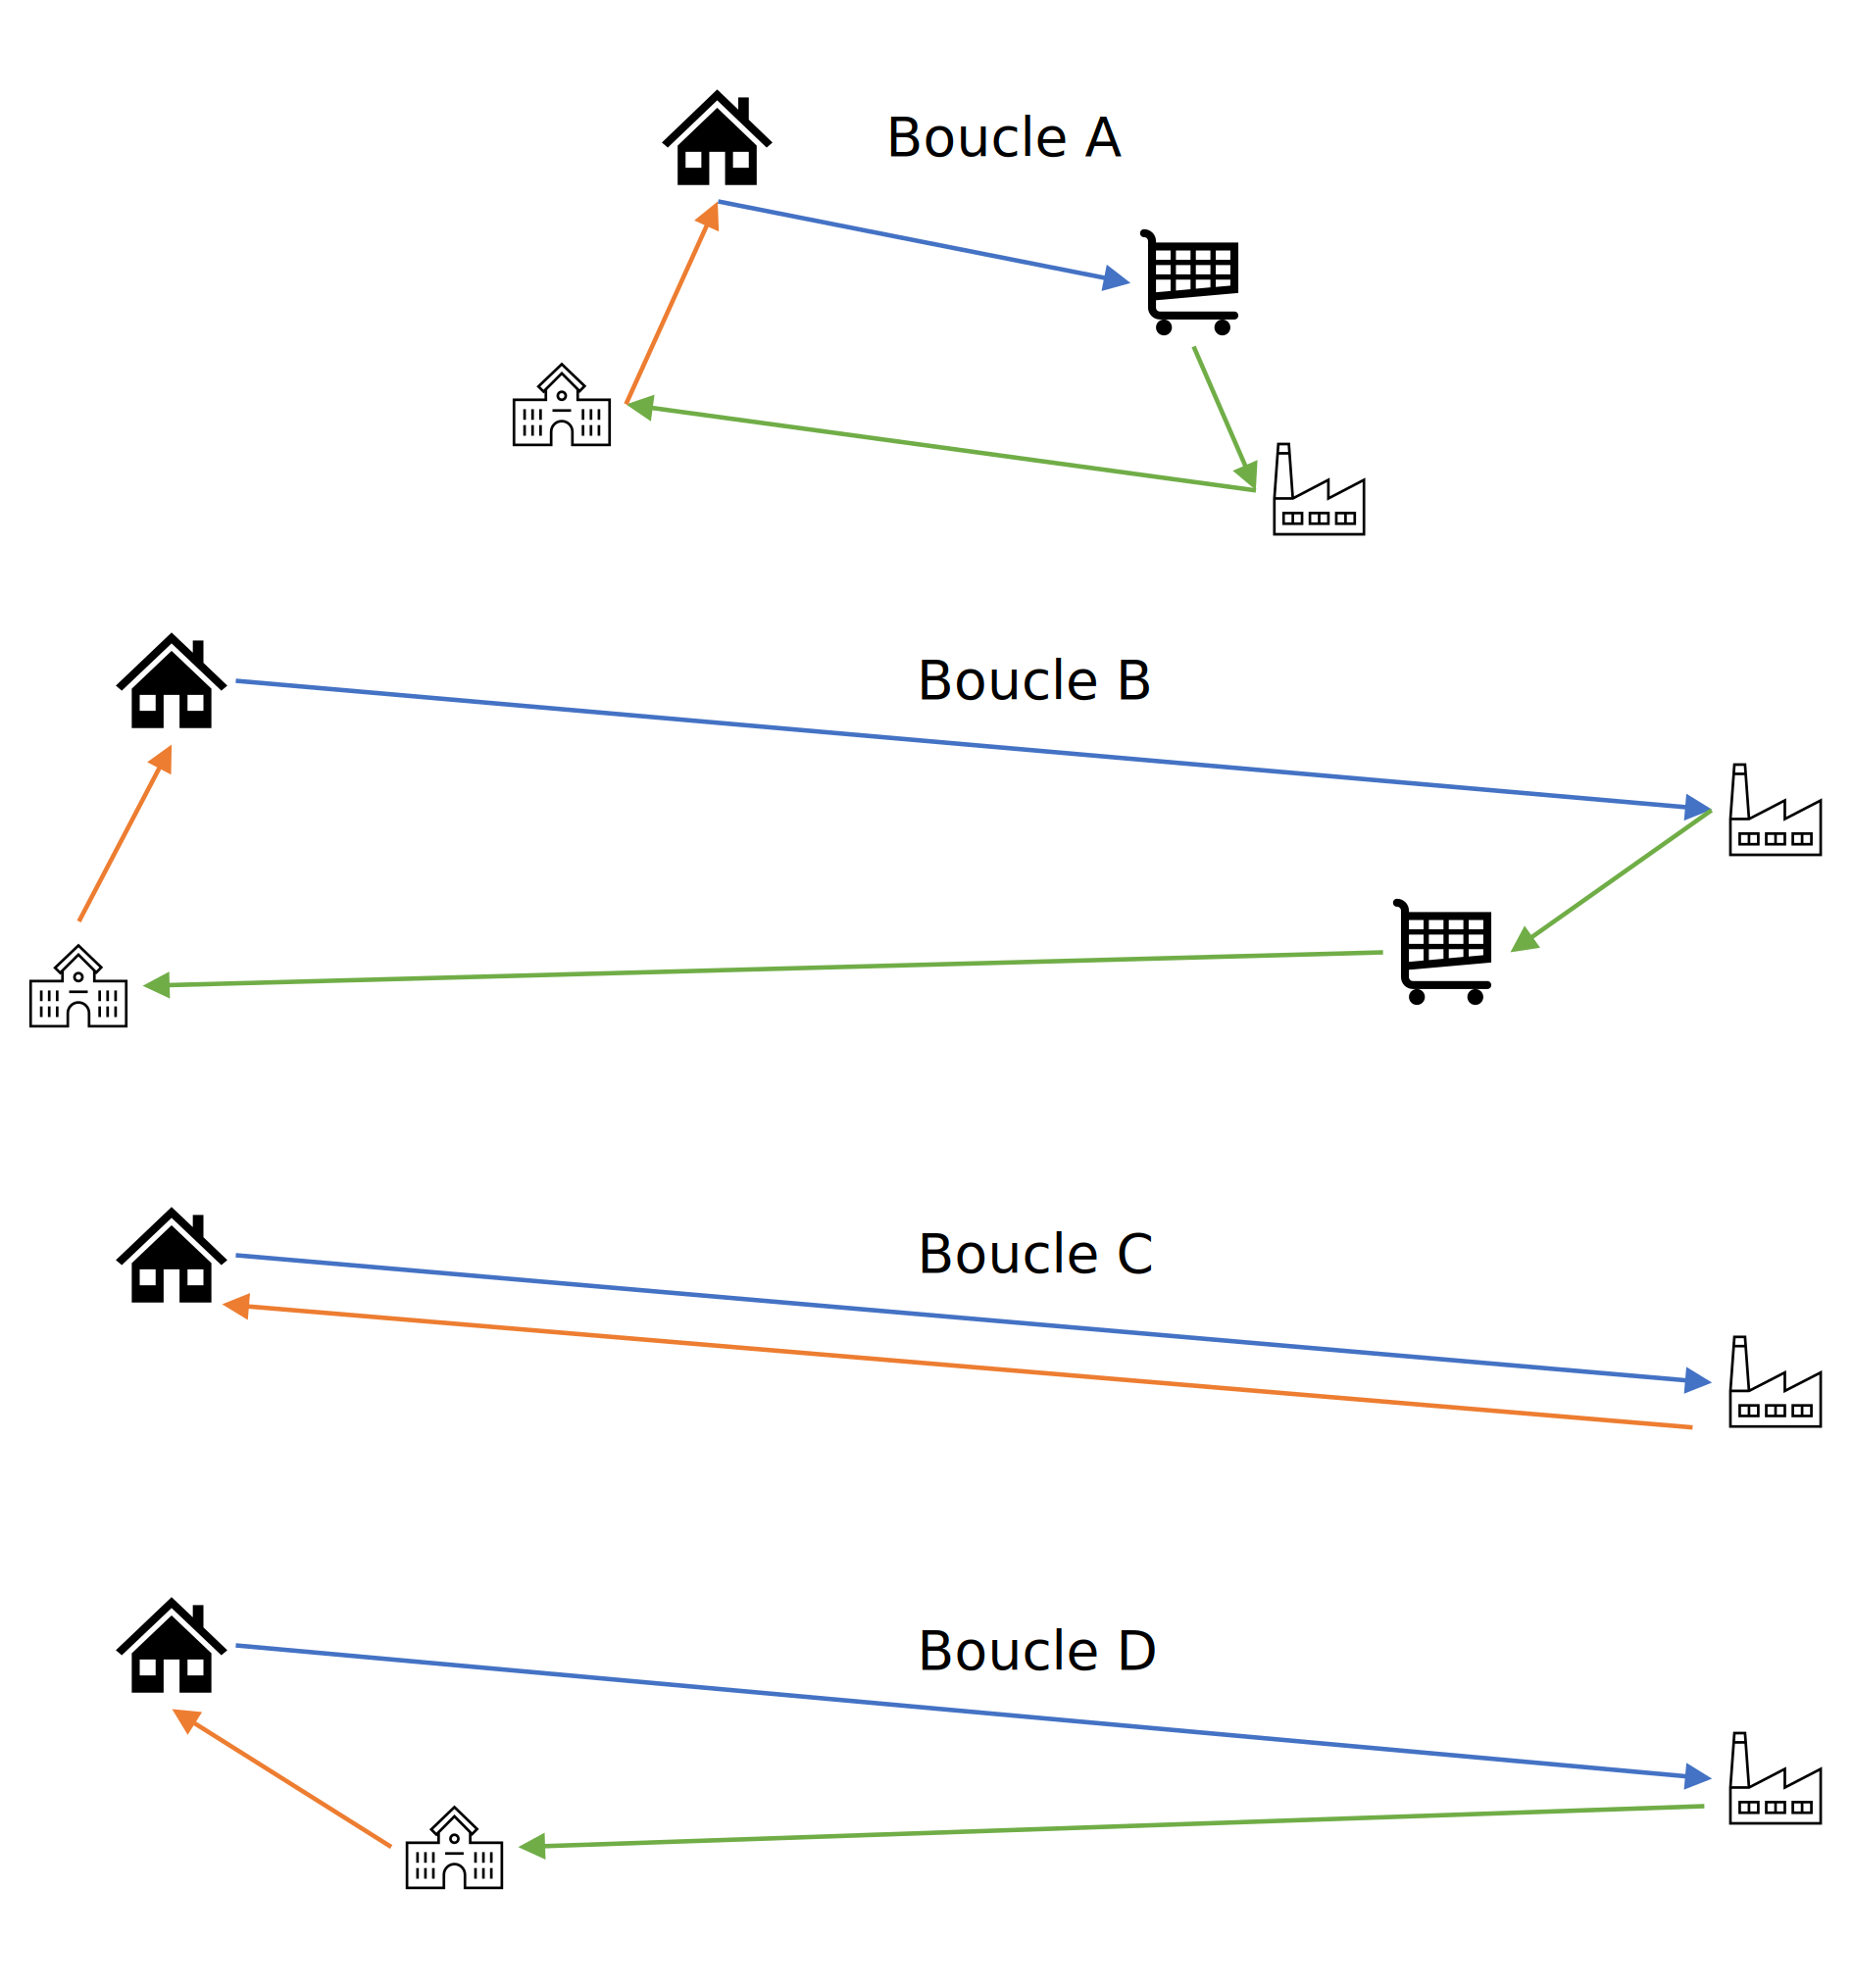
\includegraphics[width=5.20833in,height=\textheight]{trajets_files/mediabag/images/boucles.pdf}

}

\end{figure}%

En se limitant aux individus pour lesquels il a été possible d'inférer
la distance domicile-travail dans l'enquête EMP 2019, nous pouvons
estimer la proportion de détours \(\gamma\) en fonction de la distance
\(d\). La relation est de type \emph{log-log} à condition de s'écarter
des valeurs nulles, très proches de zéro ou au contraire très élevées.
La proportion du détour est parfois nulle, aussi nous avons ajouté
systématiquement 1\% à cette proportion. Les distances proches de zéro
sont également un problème puisqu'elles font diverger la proportion
estimée. Or nous voulons un modèle qui renvoie une valeur finie
raisonnable quand la distance tend vers 0. Nous avons donc ajouté 1
kilomètre à la distance dans l'équation à cet effet. Cet ajout ne
perturbe pas l'estimation pour les longues distances et permet de borner
l'effet du multiplicateur à courte distance. Nous avons également écarté
les cas où \(K\) dépassait 10. Pour ne pas faire trop dépendre nos
estimations de ces choix préalables, il fallait utiliser une méthode
robuste. Nous avons opté pour une régression par quantile, en estimant
la médiane, soit pour des individus indicés par \emph{l} :

\begin{equation}\phantomsection\label{eq-prop-detours}{
log(\gamma_l) = \alpha + \beta \times log(1 + d_l) + \varepsilon_l
\\ avec\ \varepsilon_l \sim \mathcal{N}
\\ en\ minimisant \sum_l \left\lvert{\varepsilon_l}\right\lvert
}\end{equation}

\begin{longtable}{lrrrr}

\caption{\label{tbl-reg-detours}Estimation de la proportion des détours
en fonction de la distance domicile-travail}

\tabularnewline

\toprule
term & estimate & conf.low & conf.high & tau \\ 
\midrule\addlinespace[2.5pt]
(Intercept) & 1.675790 & 1.226465 & 2.0341652 & 0.5 \\ 
log(distance + 1) & -1.070136 & -1.327079 & -0.8492878 & 0.5 \\ 
\bottomrule

\end{longtable}

Le modèle a un \(R^2\) de 0.24. Le graphique graphique~\ref{fig-dist2K}
montre l'allure de notre estimation médiane par rapport aux données
issues de l'EMP.

\begin{figure}[htb]

\caption{\label{fig-dist2K}Facteur K en fonction de la distance
domicile-travail}

\centering{

\includegraphics[width=1\textwidth,height=\textheight]{trajets_files/figure-pdf/fig-dist2K-1.png}

}

\end{figure}%

On notera que les détours sont surtout importants\,-- en proportion\,--
à faibles distances et, comme nous l'avons vu précédemment, demeurent
assez peu fréquents. L'un dans l'autre, le rôle joué par les détours
dans notre modélisation reste relativement modeste.

\section{Choix modal}\label{choix-modal}

A ce stade de notre modélisation des pratiques de mobilités, nous savons
prédire la fréquence des boucles et leur longueur. Il reste à estimer
les choix modaux des individus en fonction de leurs caractéristiques et
des caractéristiques des boucles envisagées. Pour ce faire, nous nous
sommes appuyés fort classiquement sur les modèles d'utilités aléatoires
(notés RUM par la suite, pour \emph{Random Utility Model}, McFadden
(1974)). Le principe de ces modèles est d'estimer pour chacun des modes
de transport disponibles son utilité probable en fonction de divers
paramètres comme le temps de trajet, le prix du trajet, le confort
ressenti le long du trajet ou encore les caractéristiques de l'individu
qui fera le trajet. Une des hypothèses du modèle est que les individus
ont des préférences inobservables qui font que leur préférence pour un
mode de transport vont varier aléatoirement (du point de vue de
l'observateur) d'un individu à l'autre. Ce pourquoi, pour une demande de
mobilité donnée, on estime en fait une distribution de probabilités de
l'utilité pour chacun des modes. La comparaison des distributions permet
ensuite d'estimer la probabilité d'un individu de choisir plutôt tel
mode de transport que tel autre mode.

Nous avons estimé deux modèles RUM sur les données EMP 2019\,: un modèle
avec 4 choix modaux (marche à pied, vélo, voiture, transport en commun)
et un autre avec uniquement les 3 premiers choix, pour les cas où il n'y
a pas de transport en commun envisageable pour la boucle considérée.
Pour mener à bien ces estimations, il faudrait idéalement pouvoir
renseigner aux mieux chacun des choix modaux. Or l'enquête EMP nous
renseigne essentiellement sur les caractéristiques du trajet effectif
selon le mode retenu, et non sur les caractéristiques des modes
alternatifs. En conséquence, nous n'avons mobilisé qu'une seule
caractéristique spécifique selon le mode\,: le temps de trajet. Et nous
avons dû l'inférer à partir de la vitesse moyenne de chaque mode et de
la distance parcourue. Au passage, nous avons fait l'hypothèse que la
distance parcourue est indépendante du mode, ce qui n'est pas toujours
vérifiée. Même si, sur un territoire donnée, nous pouvons estimer une
distance par mode (où, notamment, la distance à pied pourrait être
parfois plus courte que celle en voiture), de telles distinctions ne
sont pas disponibles dans EMP 2019.

En revanche, s'agissant des caractéristiques partagées entre les
différents modes, nous sommes bien moins limités. Nous avons toutefois
évacué certaines variables non pas parce qu'elles manqueraient de
pertinence, mais parce qu'elles n'induisent pas d'hétérogénéité
spatiale. Notamment, le sexe de l'individu peut jouer sur le choix
modal, mais le fait d'intégrer cet aspect dans notre modèle n'a pas
d'intérêt puisque la distribution spatiale des femmes est similaire à la
celle des hommes. Seules nous intéresse les variables qui peuvent
engendrer des différences de comportements moyens sur le territoire
\emph{par effet de composition spatiale}. Or, même si les hommes font,
par exemple, plus souvent des trajets à vélo que les femmes, cet écart
n'a pas de conséquence spatiale puisque la répartition homme-femme est
homogène sur le territoire. Nous n'avons pas pris en compte non plus
l'âge car nos estimations ont été effectuées sur les actifs uniquement.
Certes, il y a bien des différences de comportements de mobilité selon
l'âge, mais ces différences s'observent surtout entre les enfants, les
étudiants, les actifs et les retraités, plus qu'entre les actifs.

Au final, les modèles RUM estimés s'appuient sur les variables
suivantes\,: \(U_{bcl,l}^m\) est l'utilité du mode de transport \emph{m}
pour un individu \emph{l} prévoyant d'effectuer une boucle \emph{bcl},
\(tt_{bcl, m}\) le temps total des trajets pour parcourir cette boucle
dans le mode \emph{m}, \(L_bcl\) la longueur de cette boucle, \(dens_l\)
la densité de la commune de résidence (selon le code INSEE qui va de 1
pour «\,Très dense\,» à 4 pour «\,Très peu dense\,», en fusionnant les
catégories 3 et 4 car cette dernière est rare dans EMP 2019),
\(typmen_l\) le type de ménage, \(voiture_l\) le fait de posséder une
voiture (au moins) et \(NdV_l\) le niveau de vie du ménage.

Il s'agit d'estimer les fonctions d'utilités suivantes\,:

\begin{equation}\phantomsection\label{eq-utility}{
U_l^m = \alpha_m + \beta \times tt_{bcl,m} + \gamma_m \times log(L_{bcl}) + \delta_m \times log(NdV_l)
\\ \lambda_m \times dens_l + \mu_m \times typmen_l + \nu_m \times voiture_l + \varepsilon_{m,l}
\\ avec\ \varepsilon_{m,l} \sim Loi\ de\ Gumbel
}\end{equation}

Nous nous en tenons, pour l'heure, à la modélisation la plus simple en
faisant l'hypothèse que les erreurs sont distribuées selon une loi de
Gumbel, conformément à la première formulation du modèle RUM par
McFadden . Ceci revient à supposer que ces erreurs sont indépendantes et
homoscédastiques et permet de se ramener à un simple modèle logistique
multinomiale.

\begin{longtable}{lrrrr}

\caption{\label{tbl-rum-tc}Estimation des paramètres du modèle d'utilité
aléatoire avec transport en commun}

\tabularnewline

\toprule
Facteur & Coefficient estimé & Ecart type & t Student & p Value \\ 
\midrule\addlinespace[2.5pt]
(Intercept):car & $3.0$ & $1.9$ & $1.5$ & $0.1$ \\ 
(Intercept):transit & $10.6$ & $2.7$ & $3.9$ & $0.0$ \\ 
(Intercept):walk & $7.0$ & $2.2$ & $3.2$ & $0.0$ \\ 
tt & $0.0$ & $0.0$ & $-2.0$ & $0.0$ \\ 
DENSITECOM\_RESAssez dense:car & $1.0$ & $0.2$ & $5.0$ & $0.0$ \\ 
DENSITECOM\_RESAssez dense:transit & $-0.8$ & $0.3$ & $-2.8$ & $0.0$ \\ 
DENSITECOM\_RESAssez dense:walk & $0.1$ & $0.2$ & $0.4$ & $0.7$ \\ 
DENSITECOM\_RESPeu dense:car & $0.5$ & $0.2$ & $2.3$ & $0.0$ \\ 
DENSITECOM\_RESPeu dense:transit & $-3.1$ & $0.7$ & $-4.4$ & $0.0$ \\ 
DENSITECOM\_RESPeu dense:walk & $0.1$ & $0.3$ & $0.3$ & $0.8$ \\ 
ldistance:car & $0.7$ & $0.1$ & $5.0$ & $0.0$ \\ 
ldistance:transit & $0.7$ & $0.1$ & $4.9$ & $0.0$ \\ 
ldistance:walk & $-1.3$ & $0.1$ & $-11.6$ & $0.0$ \\ 
TYPMEN5Monoparent:car & $-0.8$ & $0.3$ & $-2.8$ & $0.0$ \\ 
TYPMEN5Monoparent:transit & $-0.4$ & $0.4$ & $-1.1$ & $0.3$ \\ 
TYPMEN5Monoparent:walk & $-1.2$ & $0.3$ & $-3.6$ & $0.0$ \\ 
TYPMEN5Couple sans enfant:car & $-0.4$ & $0.3$ & $-1.4$ & $0.2$ \\ 
TYPMEN5Couple sans enfant:transit & $0.0$ & $0.4$ & $0.1$ & $0.9$ \\ 
TYPMEN5Couple sans enfant:walk & $-0.8$ & $0.3$ & $-2.9$ & $0.0$ \\ 
TYPMEN5Couple avec enfant(s):car & $-0.3$ & $0.2$ & $-1.5$ & $0.1$ \\ 
TYPMEN5Couple avec enfant(s):transit & $-0.1$ & $0.3$ & $-0.4$ & $0.7$ \\ 
TYPMEN5Couple avec enfant(s):walk & $-0.8$ & $0.3$ & $-3.2$ & $0.0$ \\ 
TYPMEN5Autres:car & $-0.1$ & $0.8$ & $-0.1$ & $0.9$ \\ 
TYPMEN5Autres:transit & $1.7$ & $0.9$ & $1.9$ & $0.1$ \\ 
TYPMEN5Autres:walk & $0.0$ & $0.9$ & $0.0$ & $1.0$ \\ 
voitureTRUE:car & $2.4$ & $0.3$ & $8.0$ & $0.0$ \\ 
voitureTRUE:transit & $-1.5$ & $0.3$ & $-4.7$ & $0.0$ \\ 
voitureTRUE:walk & $0.0$ & $0.3$ & $-0.1$ & $0.9$ \\ 
lrevuce:car & $-0.4$ & $0.2$ & $-2.1$ & $0.0$ \\ 
lrevuce:transit & $-1.0$ & $0.3$ & $-3.7$ & $0.0$ \\ 
lrevuce:walk & $-0.3$ & $0.2$ & $-1.5$ & $0.1$ \\ 
\bottomrule

\end{longtable}

On peut voir dans le tableau~\ref{tbl-rum-tc} et la
graphique~\ref{fig-modale} les estimations du modèle dans le cas où il y
a des transports en commun. Le modèle à un \(R^2\) de McFadden de 0.42.
Le modèle sans la possibilité de transports en commun n'est pas très
différent.

\begin{figure}[htb]

\caption{\label{fig-modale}Part modale}

\centering{

\includegraphics[width=1\textwidth,height=\textheight]{trajets_files/figure-pdf/fig-modale-1.png}

}

\end{figure}%

\chapter{Projection du modèle sur l'agglomération de la
Rochelle}\label{projection-du-moduxe8le-sur-lagglomuxe9ration-de-la-rochelle}

Nous avons effectué la projection du modèle sur le territoire de La
Rochelle au carreau INSPIRE de 200m. La procédure consiste à appliquer
l'équation~\ref{eq-kmmod} en imputant au carreau 200m les variables
nécessaires. Ces variables sont celles qui nourrissent les différents
modèles et qui sont répertoriées dans le tableau~\ref{tbl-facteurs}.

Le graphique~\ref{fig-km-nav} montre, par exemple, l'estimation du
nombre moyen de kilomètres parcourus annuellement par un navetteur
résidant dans chaque carreau d'habitation. Comme attendu, plus l'on
s'éloigne des zones urbanisées, plus ce nombre de kilomètres augmente.
Il est d'une certaine manière une traduction chiffrée de la dépendance à
la voiture puisque, avec les modèles de comportements, nous avons pris
ici en compte l'adaptation des comportements due à l'éloignement aux
emplois.

\begin{figure}

\caption{\label{fig-km-nav}Km parcourus en voiture par un navetteur
(actif) pour ses déplacements professionnels}

\centering{

\includegraphics[width=1\textwidth,height=\textheight]{trajets_files/figure-pdf/unnamed-chunk-13-1.png}

}

\end{figure}%

En appliquant un ratio émissions de CO\textsubscript{2} aux kilomètres,
on peut construire une carte localisée des émissions de
CO\textsubscript{2}, ainsi que des analyses en variantes. Certains de
ces scénarios sont développés dans Lempérière \emph{et al.} (2023) dans
le cadre de l'application à la Rochelle.

\section{Prix, émission et
densité}\label{prix-uxe9mission-et-densituxe9}

La carte représentée sur le graphique~\ref{fig-km-nav} sert de base au
graphique~\ref{fig-prixkm}. Chaque point de ce graphique est un point de
la carte précédente. La taille du point indique le nombre d'actifs et
c'est ainsi proportionnel à la densité, puisque chaque carreau 200m a
une taille fixe (4 hectares)\,; la couleur représente le prix des
transactions immobilières au m² pour l'année 2019\,-- avec un lissage
pour tenir compte du faible échantillonage à cette résolution spatiale.
L'axe des y représente les kilomètres moyens parcourus par les actifs de
chaque carreau pour leurs déplacements professionnels. Enfin, l'axe des
x représente le niveau de vie (c'est-à-dire le revenu divisé par les
unités de consommation) moyen des ménages de chaque carreau.

La courbe en gris agrège les différents carreaux en pondérant par la
population de chaque carreau et illustre le lien entre kilomètre et
niveau de vie. Le nombre de kilomètres est le plus bas pour les ménages
les plus pauvres\,-- la contrainte budgétaire les oblige
certainement\,-- et les ménages les plus aisés\,-- dont la contrainte
budgétaire leur permet de se loger plus facilement près des emplois.
Pour les moins aisés, la façon de concilier la contrainte mobilité et la
contrainte logement est soit de vivre dans un logement plus petit, soit
de se voir solvabiliser par le logement social.

Pour un niveau de vie donné, la dispersion est très grande, mais le lien
apparaît significatif pour autant. Les classes moyennes (ni les plus
riches, ni les plus pauvres) émettent plus de CO\textsubscript{2} en
moyenne parce qu'elles vivent plus loin de l'emploi dans des zones moins
denses et dont le prix de l'immobilier résidentiel est plus bas. En ce
qui concerne les émissions de CO\textsubscript{2} liées à la mobilité
professionnelle quotidienne, sur le territoire de la Rochelle, notre
projection indique que les émissions diminuent avec le revenu sur la
partie haute de la distribution des revenus.

\begin{figure}[htb]

\caption{\label{fig-prixkm}Kilomètres, densité, prix immobiliers et
niveau de vie, La Rochelle}

\centering{

\includegraphics[width=1\textwidth,height=\textheight]{trajets_files/figure-pdf/fig-prixkm-1.png}

}

\end{figure}%

\section{Scénarios de
densification}\label{scuxe9narios-de-densification}

L'intérêt de cette modélisation ne réside pas uniquement dans le fait de
pouvoir synthétiser les pratiques de mobilités observées à une maille
fine, mais également dans la possibilité de prédire l'évolution de ces
pratiques en fonction de certains changements, de certains scénarios de
modification urbaine. Ici, pour éclairer le lien entre densité urbaine
et émission de gaz à effet de serre, nous avons simulé tout un ensemble
de scénarios de densification et estimé les conséquences sur les
kilomètres effectués en voiture par les navetteurs.

Chaque scénario a consisté en un petit «\,choc\,» démographique\,---
l'ajout de 100 actifs\,--- au sein d'un IRIS donné. Comme notre
modélisation suppose qu'il y a autant de navetteurs que d'emplois
localisés sur le territoire, il fallait également définir comment
évoluait la distribution spatiale des emplois. Nous avons considéré que
celle-ci croissait de 100 nouveaux emplois répartis à proportion de la
distribution initiale. Cette répartition d'emplois ne favorise aucun
IRIS en particulier en posant l'indépendance de l'évolution des emplois
par rapport aux IRIS. Elle est donc le plus neutre possible (puisqu'elle
est correspond à la répartition à l'entropie max) et elle est similaire
dans tous les scénarios présentés ici.

On notera que tous les IRIS ne font pas la même taille\footnote{Le plus
  petit contient 134 actifs, l'iris médian en contient 724, et le plus
  gros 2338.}. Le choc n'a donc pas le même impact localement et l'on
pourrait se demander pourquoi nous n'avons pas plutôt envisagé des chocs
migratoires proportionnels à la taille des IRIS. La raison est simple\,:
nous nous intéressons ici avant tout aux conséquences globales, plus
qu'à celles très locales, et il fallait donc mener les comparaisons en
procédant à un choc de même importance globalement. Nous regardons ainsi
comment le territoire «\,absorbe\,» ces 100 nouveaux navetteurs en
fonction de l'IRIS où ils s'installent.

On notera également qu'il y a 91\,743 navetteurs sur le territoire que
nous observons. A cet aune, 100 de plus apparaît comme un petit
«\,choc\,». Il fallait vérifier si l'ampleur du choc bouleversait nos
résultats et de quelle manière. Aussi avons-nous estimé le modèle avec
des chocs plus importants (500, 1000,\,\ldots), plus faibles (50, 10),
voire négatifs (-10, -100). Il se trouve que l'ampleur du choc ne change
pas grand chose sur le fond. En effet, notre principal élément de
comparaison entre les scénarios est le nombre annuel de kilomètres
parcourus en voiture par un résident actif sur le territoire de La
Rochelle. Au premier ordre, cette quantité est assez simple à estimer à
partir du scénario de référence (graphique~\ref{fig-km-nav})\,: si l'on
ajoute \emph{x} individus dans le carreau \emph{i} alors on peut estimer
qu'ils parcourent le nombre de kilomètres typique des résidents de ce
carreau \emph{i} dans le scénario de référence\,; il suffit alors de
recalculer la moyenne en prenant en compte les kilomètres de ces
nouveaux arrivants. Soulignons que cette propriété de quasi-linéarité
est une propriété souhaitable de notre modèle\,: l'ajout de quelques
individus ne vient pas perturber les grands équilibres et chacun se
comporte à peu près comme les autres résidents de son carreau d'arrivée.
Sans cette propriété, le modèle serait instable. Bien entendu, plus l'on
rajoute d'individus dans un carreau ou un IRIS, plus notre modèle va
finir par faire apparaître des effets non linéaires, en raison notamment
de la saturation des emplois de proximité, qui va obliger les nouveaux
venus à chercher plus loin un emploi disponible. Et c'est exactement ce
que l'on observe. Il reste que, en raison de cette quasi-linéarité,
l'ampleur du choc n'est pas un facteur décisif pour estimer les
élasticités présentées ici.

On notera enfin que les 100 actifs ajoutés ont à chaque fois les mêmes
caractéristiques sociales. Nous avons retenu comme caractéristiques de
référence celles du cas majoritaire\,: des actifs vivant en couple, avec
un ou plusieurs enfants, possédant au moins une voiture et ayant le
niveau de vie moyen du territoire. Ils ont donc le même modèle de
comportements, ce qui ne veut pas dire qu'ils auront au final les mêmes
pratiques. Selon les carreaux où ils s'installent, les pratiques seront
différentes puisque les comportements s'adaptent à la situation
géographique du carreau.

La carte du graphique~\ref{fig-elas-km-pop} fait clairement apparaître
que le nombre de kilomètres parcourus en voiture par les navetteurs sur
le territoire varie selon l'endroit où se produit la densification de
population. L'élasticité du nombre de kilomètres sur la population
totale (soit le ratio de la variation du nombre de kilomètres rapportée
à l'ampleur du choc démographique) est négative au cœur de l'aire
urbaine, dans le centre de La Rochelle, et devient positive à mesure
qu'on s'en éloigne.

\begin{figure}[htb]

\caption{\label{fig-elas-km-pop}Elasticité de km voiture sur la
population totale pour 100 nouveaux navetteurs dans l'IRIS}

\centering{

\includegraphics[width=1\textwidth,height=\textheight]{trajets_files/figure-pdf/fig-elas-km-pop-1.png}

}

\end{figure}%

Cette carte conforte l'intuition commune qui associe une forte densité
urbaine à une réduction des kilomètres parcourus en voiture et, donc,
une réduction des émissions de gaz à effet de serre. Il est possible de
préciser cette relation en examinant pour chacun des scénarios le lien
entre l'élasticité des kilomètres rapportés au choc démographique et
l'élasticité de la densité articulée (ou, terme que nous préférons, la
densité ressentie) rapportés à ce même choc démographique.

\section{De la densité aux
kilomètres}\label{de-la-densituxe9-aux-kilomuxe8tres}

Le graphique~\ref{fig-elas-km-pwd} montre l'élasticité des kilomètres
rapportés au choc démographique et l'élasticité de la densité ressentie
rapportée à ce même choc. Nous aurions pu présenter le même graphique
avec la densité urbaine au sens usuel mais, dans ce cas, le graphique
aurait été simplement moins intéressant puisque l'élasticité de la
densité urbaine est une constante dans tous les scénarios. Ce graphique
aurait été unidimensionnel en écrasant la dispersion selon l'axe des
abscisses. Mais il aurait fourni la même information sur l'élasticité
des kilomètres parcourus en voiture sur la population.

Comme on peut le constater sur le graphique~\ref{fig-elas-km-pwd},
l'élasticité des kilomètres peut être aussi bien positive que négative.
Pour un même choc démographique, une même variation de la densité
urbaine, on peut avoir une dégradation du bilan kilométrique ou une
amélioration. Une densification\,-- au sens usuel\,-- dans un des IRIS
situés en haut du graphique conduit à dégrader le bilan kilométrique. Il
s'agit des IRIS correspondant aux communes rurales, celles qui ont été
identifiées comme éloignés des emplois. Et, inversement, une
densification dans un des IRIS du bas du graphique améliore le bilan
kilométrique par actif.

Il est intéressant de relier cette simple analyse aux variations de
l'élasticité de la densité ressentie\footnote{La densité urbaine au sens
  classique se contente de faire une moyenne sur des unités spatiales au
  lieu de faire une moyenne sur des individus. Or, ce qui nous importe,
  c'est la densité autour de chaque individu. On peut l'illustrer
  simplement par le cas de deux unités spatiales où résident 10
  individus. La densité urbaine usuelle est de 5 dans tous les cas.
  Pourtant, ce n'est pas la même chose de se répartir entre les deux
  unités spatiales en deux groupes égaux de 5 et 5 ou, par exemple, en
  un groupe de 9 et un de 1. Dans le premier cas, il y a dans chaque
  unité 5 individus qui cohabitent avec 5 individus (lui compris)\,:
  chacun perçoit une densité de 5 et la moyenne est donc de 5. Dans le
  dernier cas, ce sont 9 individus qui vivent auprès de 8 autres (plus
  lui-même), et 1 qui vit seul. Cette fois, on a 9 contributions à la
  densité qui s'élèvent à 9, soit 81, et une contribution qui vaut 1. La
  densité moyenne est de 8,2. Techniquement, la densité ressentie, c'est
  l'espérance de densité pour un individu pris au hasard\,; la densité
  urbaine, c'est l'espérance de densité pour une unité spatiale prise au
  hasard.}. On observe tout d'abord que l'élasticité de la densité peut
être négative. En effet, lorsque l'on augmente le nombre d'individu dans
une zone peu dense, deux effets contradictoires se combinent\,: d'un
côté, on augmente la densité de cette zone, mais d'un autre côté, on
augmente la probabilité qu'un individu pris au hasard soit un individu
de cette zone peu dense, ce qui a pour effet de diminuer l'espérance de
densité. Quand ce deuxième effet domine, la densité ressentie diminue.
C'est ce qui se produit pour une partie des IRIS situés en haut du
graphique\,: le choc démographique augmente le nombre de ruraux et
diminue la densité ressentie. Pour ces IRIS, le bilan kilométrique se
dégrade.

Dans le cadran en bas à droite du graphique, on a une autre composante
attendue du lien entre densité et KVT\,: un choc démographique dans un
IRIS très urbanisé\,-- ici, le centre de La Rochelle\,-- provoque à la
fois une claire augmentation de la densité ressentie et une amélioration
du bilan kilométrique par actif.

Il y a enfin un dernier cadran non vide, situé en bas à gauche, où le
choc démographique n'a pas d'impact fort sur la densité ressentie tout
en améliorant le bilan. Il s'agit de la première couronne autour de La
Rochelle. Ainsi, un choc démographique dans cette zone précise a la
particularité de ne pas être ressentie comme une densification tout en
permettant une forte réduction des émissions de gaz à effet de serre. De
nombreux opposants à la densification associent celle-ci à l'image de
résidents entassées dans des tours, image qu'ils jugent repoussante. Or
ce cadran montre qu'il existe des formes de densification écologique qui
ne sont pas ressenties comme des fortes densifications.

\begin{figure}[htb]

\caption{\label{fig-elas-km-pwd}Elasticité de km voiture en fonction de
la densité ressentie}

\centering{

\subcaption{\label{fig-elas-km-pwd}pour un choc démographique ciblé dans
un IRIS}

\centering{

\includegraphics[width=1\textwidth,height=\textheight]{trajets_files/figure-pdf/fig-elas-km-pwd-1.png}

}

}

\end{figure}%

\chapter*{Références
bibliographiques}\label{ruxe9fuxe9rences-bibliographiques}
\addcontentsline{toc}{chapter}{Références bibliographiques}

\phantomsection\label{refs}
\begin{CSLReferences}{0}{1}
\bibitem[\citeproctext]{ref-batty2013}
Batty M. (2013).
\emph{\href{https://doi.org/10.7551/mitpress/9399.001.0001}{The New
Science of Cities}}, The MIT Press.

\bibitem[\citeproctext]{ref-empreinte2022}
Baude M. (2022).
{«~\href{https://www.statistiques.developpement-durable.gouv.fr/sites/default/files/2022-07/document_travail_59_decomposition_empreinte_carbone_juillet2022.pdf}{La
décomposition de l'empreinte carbone de la demande finale de la France
par postes de consommation : transport, alimentation, habitat,
équipements et services}~»}, \emph{document de travail}, 59, Ministère
de la transition écologique et de la cohésion des territoires.

\bibitem[\citeproctext]{ref-bettencourt2021}
Bettencourt L. (2021).
\emph{\href{https://doi.org/10.7551/mitpress/13909.001.0001}{Introduction
to Urban Science: Evidence and Theory of Cities as Complex Systems}}.

\bibitem[\citeproctext]{ref-blaudindethuxe92021}
Blaudin de Thé C., Carantino B., Lafourcade M. (2021).
{«~\href{https://doi.org/10.1016/j.regsciurbeco.2021.103693}{The carbon
{`}carprint{'} of urbanization: New evidence from French cities}~»},
\emph{Regional Science and Urban Economics}, \emph{89}, p.~103693.

\bibitem[\citeproctext]{ref-brownstone2009}
Brownstone D., Golob T.F. (2009).
{«~\href{https://doi.org/10.1016/j.jue.2008.09.002}{The impact of
residential density on vehicle usage and energy consumption}~»},
\emph{Journal of Urban Economics}, \emph{65}, n° 1, p.~91‑98.

\bibitem[\citeproctext]{ref-cervero1989}
Cervero R. (1989).
{«~\href{https://doi.org/10.1080/01944368908976014}{Jobs-Housing
Balancing and Regional Mobility}~»}, \emph{Journal of the American
Planning Association}, \emph{55}, n° 2, p.~136‑150.

\bibitem[\citeproctext]{ref-cervero1997}
Cervero R., Kockelman K. (1997).
{«~\href{https://doi.org/10.1016/S1361-9209(97)00009-6}{Travel demand
and the 3Ds: Density, diversity, and design}~»}, \emph{Transportation
Research Part D: Transport and Environment}, \emph{2}, n° 3, p.~199‑219.

\bibitem[\citeproctext]{ref-Conway1962}
Conway R.W., Maxwell W.L. (1962). {«~A queuing model with state
dependent service rates~»}, \emph{Journal of Industrial Engineering},
\emph{12}, n° 2, p.~132‑136.

\bibitem[\citeproctext]{ref-dantzig1973}
Dantzig G.B., Dantzig G.B., Saaty T.L. (1973).
\emph{\href{https://books.google.fr/books?id=PTeIQgAACAAJ}{Compact City:
A Plan for a Liveable Urban Environment}}, W. H. Freeman.

\bibitem[\citeproctext]{ref-duranton2018}
Duranton G., Turner M.A. (2018).
{«~\href{https://doi.org/10.1016/j.jue.2018.10.003}{Urban form and
driving: Evidence from US cities}~»}, \emph{Journal of Urban Economics},
\emph{108}, p.~170‑191.

\bibitem[\citeproctext]{ref-ewing1997}
Ewing R. (1997). {«~\href{https://doi.org/10.1080/01944369708975728}{Is
Los Angeles-Style Sprawl Desirable?}~»}, \emph{Journal of the American
Planning Association}, \emph{63}, n° 1, p.~107‑126.

\bibitem[\citeproctext]{ref-ewing2010}
Ewing R., Cervero R. (2010).
{«~\href{https://doi.org/10.1080/01944361003766766}{Travel and the Built
Environment}~»}, \emph{Journal of the American Planning Association},
\emph{76}, n° 3, p.~265‑294.

\bibitem[\citeproctext]{ref-ewing2015}
Ewing R., Hamidi S. (2015).
{«~\href{https://doi.org/10.1177/0885412215595439}{Compactness versus
Sprawl: A Review of Recent Evidence from the United States}~»},
\emph{Journal of Planning Literature}, \emph{30}, n° 4, p.~413‑432.

\bibitem[\citeproctext]{ref-ewing2017}
Ewing R., Hamidi S., Tian G., Proffitt D., Tonin S., Fregolent L.
(2017). {«~\href{https://doi.org/10.1177/0739456X16688767}{Testing
Newman and Kenworthy{'}s Theory of Density and Automobile
Dependence}~»}, \emph{Journal of Planning Education and Research},
\emph{38}, p.~0739456X1668876.

\bibitem[\citeproctext]{ref-gaignuxe92012}
Gaigné C., Riou S., Thisse J.-F. (2012).
{«~\href{https://doi.org/10.1016/j.jue.2012.04.001}{Are compact cities
environmentally friendly?}~»}, \emph{Journal of Urban Economics},
\emph{72}, n° 2-3, p.~123‑136.

\bibitem[\citeproctext]{ref-gordon1997}
Gordon P., Richardson H.W. (1997).
{«~\href{https://doi.org/10.1080/01944369708975727}{Are Compact Cities a
Desirable Planning Goal?}~»}, \emph{Journal of the American Planning
Association}, \emph{63}, n° 1, p.~95‑106.

\bibitem[\citeproctext]{ref-grazi2008}
Grazi F., Bergh J.C.J.M.V.D., Ommeren J.N.V. (2008).
{«~\href{https://doi.org/10.5547/ISSN0195-6574-EJ-Vol29-No4-5}{An
Empirical Analysis of Urban Form, Transport, and Global Warming}~»},
\emph{The Energy Journal}, \emph{29}, n° 4.

\bibitem[\citeproctext]{ref-handbook2007}
\textsc{Hensher, D.A.}, \textsc{Button, K.J.} (dirs.) (2007).
{«~\href{https://doi.org/10.1108/9780857245670}{Handbook of Transport
Modelling}~»}, \emph{Handbooks in Transport}.

\bibitem[\citeproctext]{ref-hirt2012}
Hirt S. (2012). {«~\href{https://doi.org/10.1177/0885412212451029}{Mixed
Use by Default: How the Europeans (Don{'}t) Zone}~»}, \emph{Journal of
Planning Literature}, \emph{27}, n° 4, p.~375‑393.

\bibitem[\citeproctext]{ref-holden2005}
Holden E., Norland I.T. (2005).
{«~\href{https://doi.org/10.1080/00420980500332064}{Three Challenges for
the Compact City as a Sustainable Urban Form: Household Consumption of
Energy and Transport in Eight Residential Areas in the Greater Oslo
Region}~»}, \emph{Urban Studies}, \emph{42}, n° 12, p.~2145‑2166.

\bibitem[\citeproctext]{ref-holian2020}
Holian M.J. (2020).
{«~\href{https://doi.org/10.1016/j.econlet.2019.108763}{The impact of
urban form on vehicle ownership}~»}, \emph{Economics Letters},
\emph{186}, p.~108763.

\bibitem[\citeproctext]{ref-hsu2023}
Hsu D., Andrews C.J., T. Han A., G. Loh C., C. Osland A., P. Zegras C.
(2023). {«~\href{https://doi.org/10.1177/08854122221097977}{Planning the
Built Environment and Land Use Towards Deep Decarbonization of the
United States}~»}, \emph{Journal of Planning Literature}, \emph{38}, n°
3, p.~426‑441.

\bibitem[\citeproctext]{ref-C200}
INSEE (2022a).
{«~\href{https://www.insee.fr/fr/statistiques/6214811?sommaire=6215217}{Revenus,
pauvreté et niveau de vie en 2017 - Données carroyées. Dispositif
Fichier localisé social et fiscal (Filosofi)}~»},.

\bibitem[\citeproctext]{ref-MOBPRO}
INSEE (2022b).
{«~\href{https://www.insee.fr/fr/statistiques/6454112}{Mobilités
professionnelles en 2019 : déplacements domicile - lieu de travail
Recensement de la population - Base flux de mobilité}~»},.

\bibitem[\citeproctext]{ref-jacobs1961}
Jacobs J. (1961).
\emph{\href{https://books.google.fr/books?id=5FdHAAAAMAAJ}{The Death and
Life of Great American Cities}}, Vintage Books (A Vintage livre).

\bibitem[\citeproctext]{ref-jenks1996}
Jenks M., Williams K., Burton E. (1996). {«~A Sustainable Future through
the Compact City? Urban Intensification in the United Kingdom~»},
\emph{Environments by Design}, \emph{1}, p.~5‑20.

\bibitem[\citeproctext]{ref-thecomp2003}
\textsc{Jenks, M.}, \textsc{Williams, K.}, \textsc{Burton, E.} (dirs.)
(2003). {«~\href{https://doi.org/10.4324/9780203362372-12}{The Compact
City: A Successful, Desirable and Achievable Urban Form?}~»}, dans
Routledge, p.~54‑65.

\bibitem[\citeproctext]{ref-lee2020}
Lee S., Lee B. (2020).
{«~\href{https://doi.org/10.1016/j.jtrangeo.2020.102694}{Comparing the
impacts of local land use and urban spatial structure on household VMT
and GHG emissions}~»}, \emph{Journal of Transport Geography}, \emph{84},
p.~102694.

\bibitem[\citeproctext]{ref-lempuxe9riuxe8re2023}
Lempérière P., Miet D., Parodi M., Pouvreau L., Stulhfauth V., Timbeau
X. (2023).
{«~\href{https://publications.vv.energy/la-rochelle-aunis-carbone.html}{SCoT
La Rochelle Aunis : les émissions moyennes des habitants du territoire
pour leurs mobilités quotidiennes}~»},.

\bibitem[\citeproctext]{ref-levine2010}
Levine J. (2010).
\emph{\href{https://books.google.fr/books?id=HTCl9W9rg3oC}{Zoned Out:
Regulation, Markets, and Choices in Transportation and Metropolitan Land
Use}}, Taylor \& Francis.

\bibitem[\citeproctext]{ref-lwasas.2022}
Lwasa, S., Seto K.C., Bai X., Blanco H., Gurney K.R., Kılkış Ş., Lucon
O., Murakami J., Pan J., Sharifi A., Yamagata Y. (2022).
{«~\href{https://www.ipcc.ch/report/ar6/wg3/downloads/report/IPCC_AR6_WGIII_Chapter08.pdf}{Urban
Systems and Other Settlements}~»}, dans Cambridge University Press,
Cambridge, UK; New York, NY, USA.

\bibitem[\citeproctext]{ref-masson2014}
Masson V., Marchadier C., Adolphe L., Aguejdad R., Avner P., Bonhomme
M., Bretagne G., Briottet X., Bueno B., Munck C. de, Doukari O.,
Hallegatte S., Hidalgo J., Houet T., Le Bras J., Lemonsu A., Long N.,
Moine M.-P., Morel T., Nolorgues L., Pigeon G., Salagnac J.-L., Viguié
V., Zibouche K. (2014).
{«~\href{https://doi.org/10.1016/j.uclim.2014.03.004}{Adapting cities to
climate change: A systemic modelling approach}~»}, \emph{Urban Climate},
\emph{10}, p.~407‑429.

\bibitem[\citeproctext]{ref-massot2007}
Massot M.-H., Orfeuil J.-P. (2007).
{«~\href{https://doi.org/10.3406/aru.2007.2710}{La contrainte
énergétique doit-elle réguler la ville ou les véhicules ? Mobilités
urbaines et réalisme écologique}~»}, \emph{Les Annales de la Recherche
Urbaine}, \emph{103}, n° 1, p.~18‑29.

\bibitem[\citeproctext]{ref-mcfadden1974d}
McFadden D. (1974).
{«~\href{https://doi.org/10.1016/0047-2727(74)90003-6}{The measurement
of urban travel demand}~»}, \emph{Journal of Public Economics},
\emph{3}, n° 4, p.~303‑328.

\bibitem[\citeproctext]{ref-munafuxf22017}
Munafò S. (2017). {«~\href{https://doi.org/10.4000/cybergeo.28634}{Forme
urbaine et mobilités de loisirs : l{'}« effet barbecue » sur le
grill}~»}, \emph{Cybergeo: European Journal of Geography}.

\bibitem[\citeproctext]{ref-muuxf1iz2013}
Muñiz I., Calatayud D., Dobaño R. (2013).
{«~\href{https://doi.org/10.1016/j.landurbplan.2013.02.004}{The
compensation hypothesis in Barcelona measured through the ecological
footprint of mobility and housing}~»}, \emph{Landscape and Urban
Planning}, \emph{113}, p.~113‑119.

\bibitem[\citeproctext]{ref-newman1989b}
Newman P., Kenworthy J. (1989b). \emph{Cities and Automobile
Dependence}, Gower Technical, Brookfield.

\bibitem[\citeproctext]{ref-newman1989a}
Newman P., Kenworthy J. (1989a).
{«~\href{https://doi.org/10.1080/01944368908975398}{Gasoline Consumption
and Cities}~»}, \emph{Journal of the Amrican Planning Association},
\emph{Winter 1989}, p.~24‑37.

\bibitem[\citeproctext]{ref-newman1999}
Newman P., Kenworthy J. (1999). \emph{Sustainability and Cities:
Overcoming Automobile Dependence}, Island Press.

\bibitem[\citeproctext]{ref-orfeuil2002}
Orfeuil J.-P., Soleyret D. (2002).
{«~\href{https://doi.org/10.1016/S0761-8980(02)00013-4}{Quelles
interactions entre les marchés de la mobilité à courte et à longue
distance~?}~»}, \emph{Recherche - Transports - Sécurité}, \emph{76},
p.~208‑221.

\bibitem[\citeproctext]{ref-pan2009}
Pan H., Shen Q., Zhang M. (2009).
{«~\href{https://doi.org/10.1177/0042098008099355}{Influence of Urban
Form on Travel Behaviour in Four Neighbourhoods of Shanghai}~»},
\emph{Urban Studies}, \emph{46}, n° 2, p.~275‑294.

\bibitem[\citeproctext]{ref-meaps2023}
Parodi M., Timbeau X. (2023).
{«~\href{https://preview.meaps.fr/theorie.html}{MEAPS : modéliser les
flux de navetteurs}~»}, \emph{Document de travail de l'OFCE}, n°
11-2023.

\bibitem[\citeproctext]{ref-patrickbonnel2001}
Patrick Bonnel (2001). \emph{Prévision de la demande de transport},
thèse de doctorat, Lyon, France.

\bibitem[\citeproctext]{ref-rodier2009}
Rodier C. (2009). {«~\href{https://doi.org/10.3141/2132-01}{Review of
International Modeling Literature: Transit, Land Use, and Auto Pricing
Strategies to Reduce Vehicle Miles Traveled and Greenhouse Gas
Emissions}~»}, \emph{Transportation Research Record}, \emph{2132}, n° 1,
p.~1‑12.

\bibitem[\citeproctext]{ref-savini2022}
Savini F., Ferreira A., von Schönfeld K.C. (2022).
\emph{\href{https://doi.org/10.4324/9781003160984}{Post-Growth
Planning}}, Routledge.

\bibitem[\citeproctext]{ref-MOBPERS}
SDES (2021).
{«~\href{https://www.statistiques.developpement-durable.gouv.fr/resultats-detailles-de-lenquete-mobilite-des-personnes-de-2019}{EMP
2019 Résultats détaillés de l'enquête mobilité des personnes de
2019}~»},.

\bibitem[\citeproctext]{ref-seto2014}
Seto K.C., Dhakal S., Bigio A., Blanco H., Delgado G.C., Dewar D., Huang
L., Inaba A., Kansal A., Lwasa S., McMahon J., Müller D.B., Murakami J.,
Nagendra H., Ramaswami A., Bento A., Betsill M., Bulkeley H., Chavez A.,
Christensen P., Creutzig F., Fragkias M., Güneralp B., Jiang L.,
Marcotullio P., McCollum D., Millard-Ball A., Pichler P., Salat S.,
Tacoli C., Weisz H., Zwickel T., Cervero R., Martinez J.T. (2014).
{«~\href{https://www.ipcc.ch/site/assets/uploads/2018/02/ipcc_wg3_ar5_chapter12.pdf}{12
Human Settlements, Infrastructure, and Spatial Planning}~»}, dans
Cambridge University Press, Cambridge, United Kingdom; New York, NY,
USA.

\bibitem[\citeproctext]{ref-simini2012}
Simini F., González M.C., Maritan A., Barabási A.-L. (2012).
{«~\href{https://doi.org/10.1038/nature10856}{A universal model for
mobility and migration patterns}~»}, \emph{Nature}, \emph{484}, n° 7392,
p.~96‑100.

\bibitem[\citeproctext]{ref-stevens2017}
Stevens M.R. (2017).
{«~\href{https://www.tandfonline.com/doi/epdf/10.1080/01944363.2016.1240044?needAccess=true&role=button}{Does
Compact Development Make People Drive Less?}~»}, \emph{Journal of the
American Planning Association}, \emph{38}, n° 1, p.~7‑17.

\bibitem[\citeproctext]{ref-stouffer1940}
Stouffer S.A. (1940).
{«~\href{https://doi.org/10.2307/2084520}{Intervening Opportunities: A
Theory Relating Mobility and Distance}~»}, \emph{American Sociological
Review}, \emph{5}, n° 6, p.~845.

\bibitem[\citeproctext]{ref-thurner2018}
Thurner S., Klimek P., Hanel R. (2018).
\emph{\href{https://doi.org/10.1093/oso/9780198821939.001.0001}{Introduction
to the Theory of Complex Systems}}, Oxford University Press.

\bibitem[\citeproctext]{ref-tukey77}
Tukey J.W. (1977). \emph{Exploratory Data Analysis}, Addison-Wesley.

\end{CSLReferences}



\end{document}
